\chapter{Wstęp}
	\section{Cel}
	Celem pracy inżynierskiej jest budowa środowiska symulacyjnego robota mobilnego z kołami szwedzkimi.
	Dla realizacji tego celu należy opracować model 3D, oraz model dynamiki dookólnej bazy jezdnej z 4 kołami szwedzkimi.
	Jednym z przyjętych założeń jest wymaganie, aby opracowany model był możliwie dokładny i jego działanie było zbliżone do rzeczywistego robota.
	Opisywana platforma będzie używana jako baza wielokierunkowa do przemieszczania dwuramiennego robota manipulacyjnego Velma.

	Celem jest stworzenie modelu, który będzie reagował na siły podobnie do rzeczywistego robota i był sterowany tak samo, jak rzeczywisty robot.
	To spowoduje, że możliwe będzie stworzenie jednego wspólnego programu sterującego do użycia zarówno w symulacji, jak i rzeczywistym robocie.

	Testowanie oprogramowania sterującego na rzeczywistym obiekcie może prowadzić do jego uszkodzeń, 
	dlatego wpierw należy się upewnić o poprawności projektowanych rozwiązań na bezpiecznym modelu wirtualnym.
	Rzeczywistość nie pozwala także na skomplikowane scenariusze testów, które w rzeczywistości mogłyby być niemożliwe do wykonania lub koszty jego wykonania byłyby zbyt wysokie.
	Szybciej i taniej jest stworzyć symulacyjne środowisko testowe, niż fizyczne, w dodatku błąd sterowników przy symulacji nie grozi zniszczeniem rzeczywistego robota.
	Dopiero przy osiągnięciu satysfakcjonującej jakości sterowania w symulacji wirtualnej, 
	można zastosować algorytmy sterowania do rzeczywistego obiektu bez ryzyka uszkodzeń urządzenia.

	Oprócz modelu bazy jezdnej, środowisko symulacyjne musi również udostępniać modele czujników, w które wyposażony jest robot. 
	Odczyty z symulatorów czujników są następnie wykorzystywane w układzie sterowania do generacji odpowiednich sygnałów sterujących.
	W celu możliwie wiernej symulacji działania czujników, do wartości pomiarów dodaje się szum pomiarowy i zakłócenia.


\section{Dookólna platforma mobilna}
	\begin{figure}[H]
	\centering
	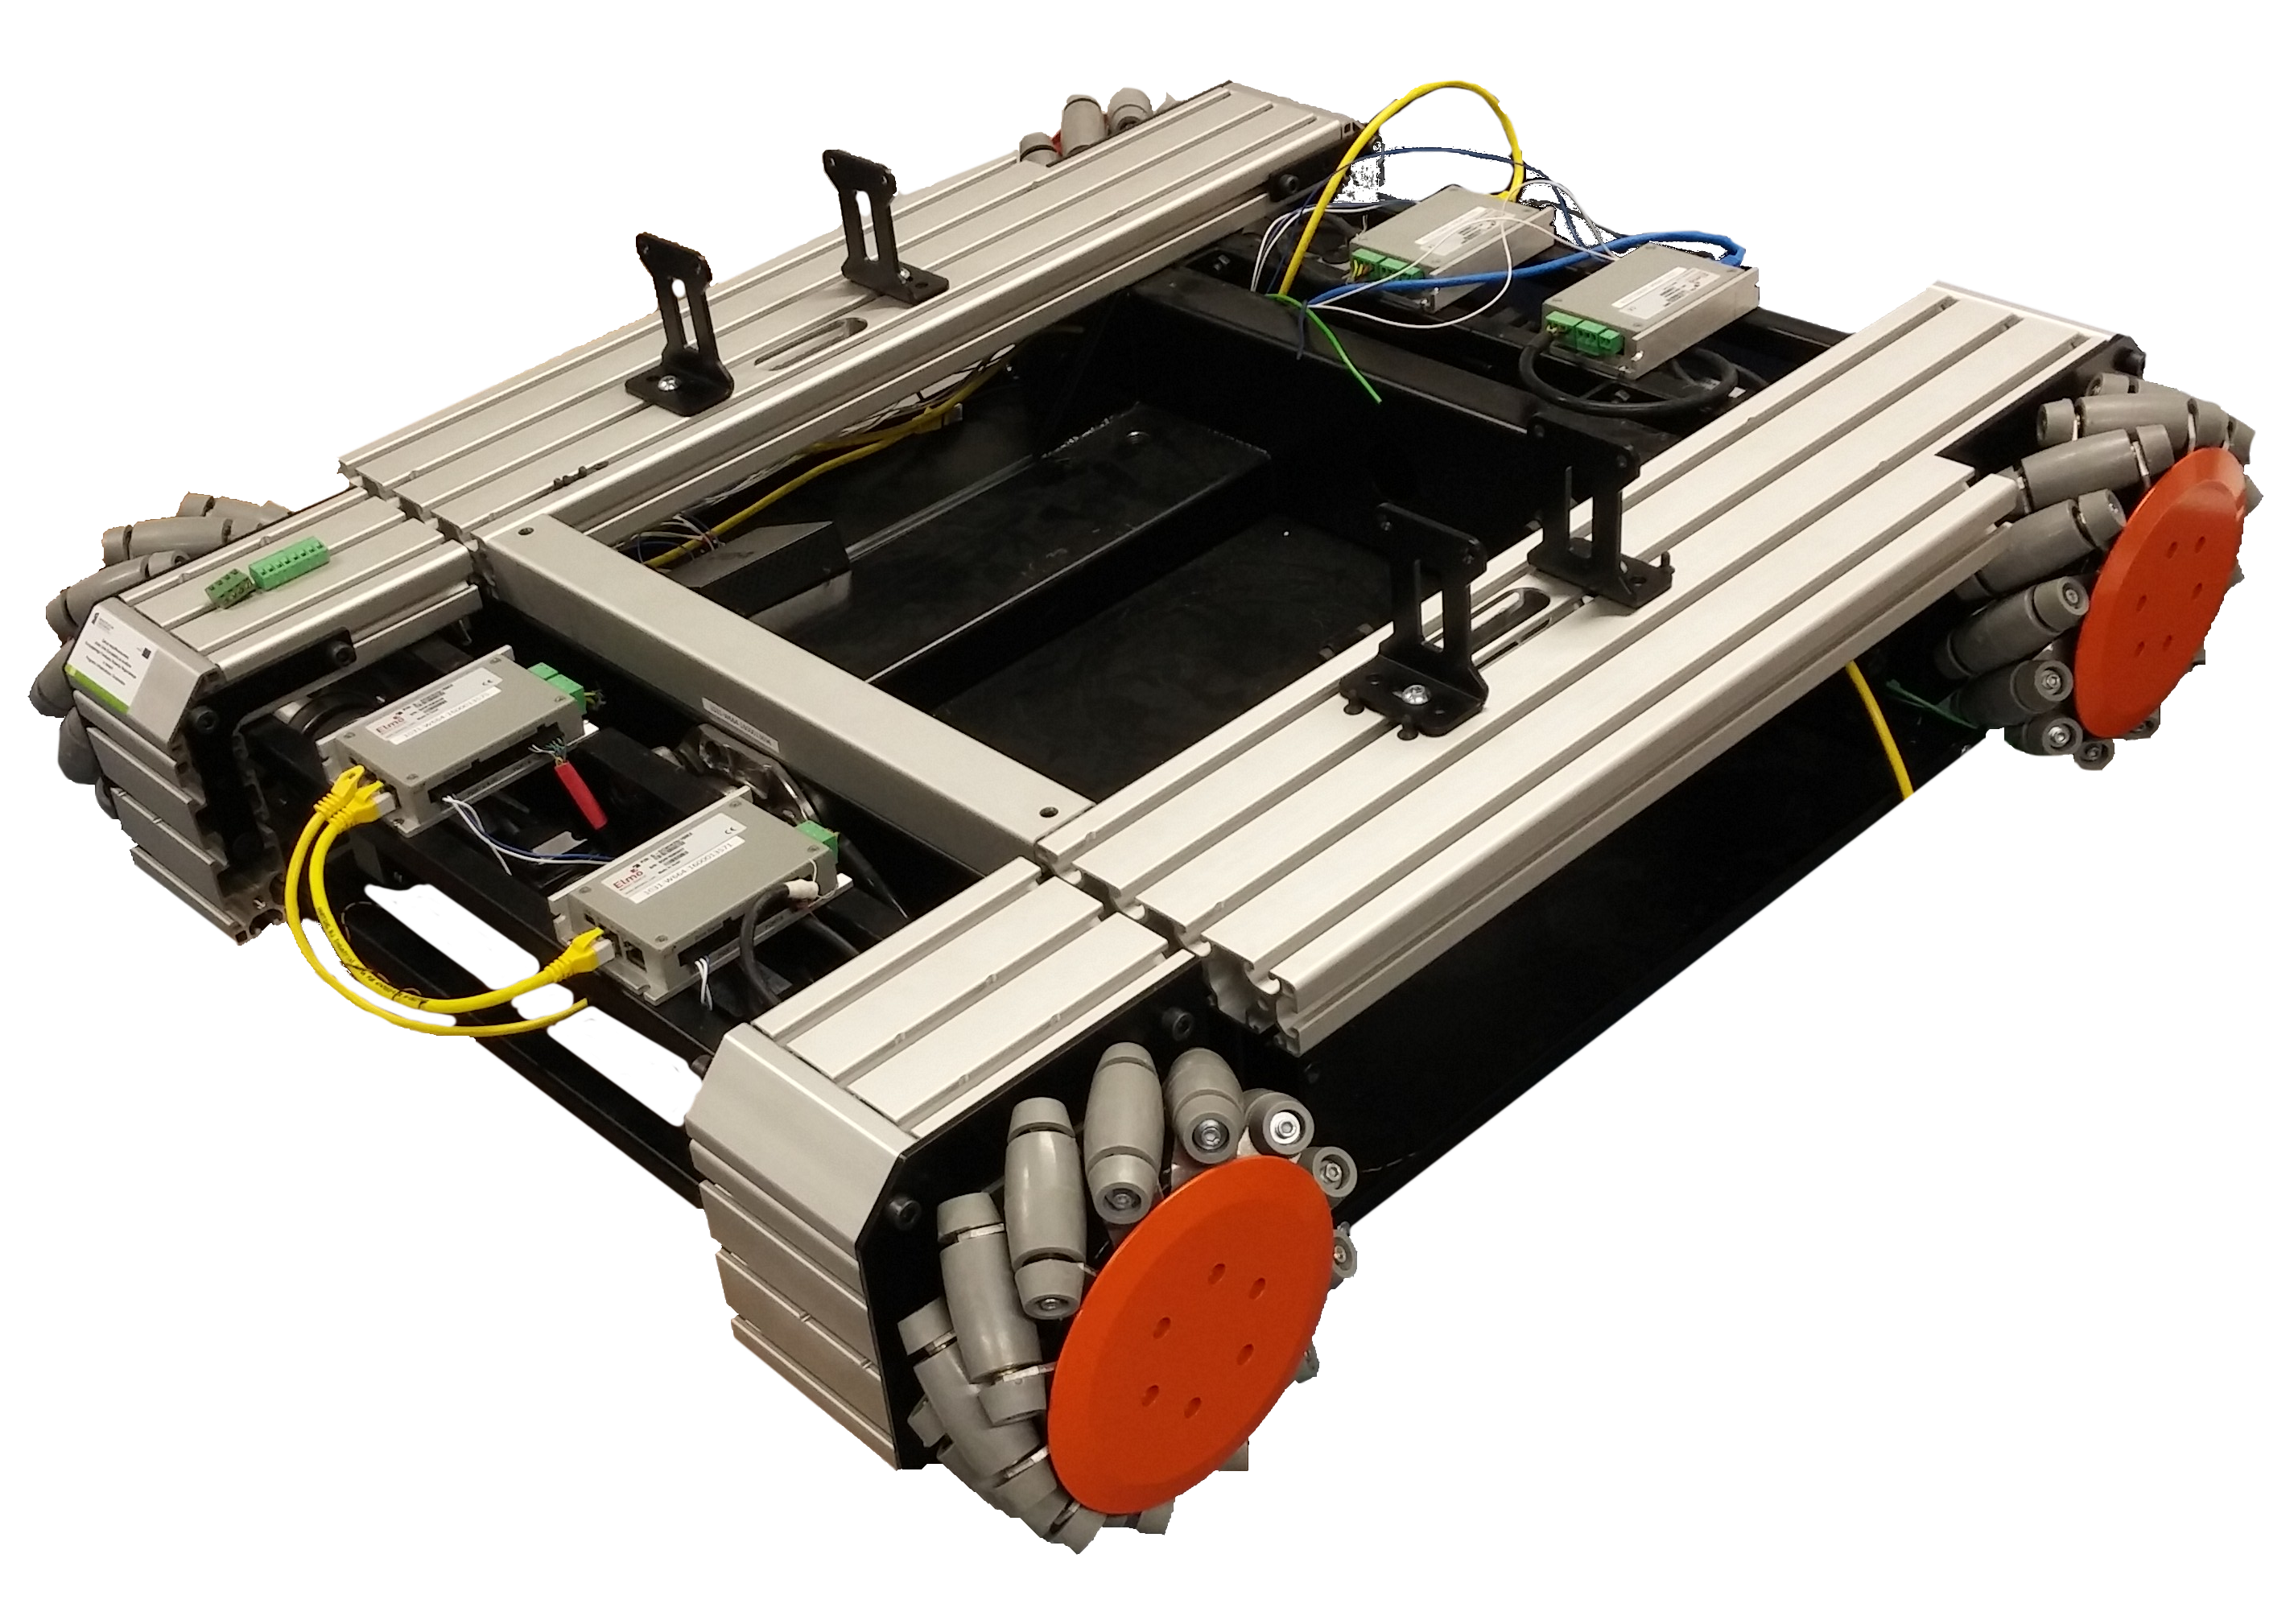
\includegraphics[width=0.8\textwidth]{graphics/base_photo.png}
	\caption{Dookólna baza mobilna na kołach szwedzkich.}
	\label{fig:base_photo}
	\end{figure} 

	Jest to duża, prostokątna baza dookólna poruszająca się na czterech kołach szwedzkich, patrz fotografia \ref{fig:base_photo}.
	Koła są stałe, parami przytwierdzone do dwóch osi.
	Każde koło jest sterowane osobno przez podłączony bezpośrednio serwomotor, 
	zatem może mieć prędkość i kierunek niezależny od prędkości pozostałych kół, kierunku poruszania się robota, oraz jego obrotu.
	Każdy z serwomotorów ma także wbudowany enkoder.
	Sterownik enkodera zwraca aktualny kąt i prędkość obrotu.

	Jest to najpopularniejsza budowa dookólnych platform mobilnych, mająca zastosowanie także w innych robotach, jak na przykład Kuka Youbot \ref{fig:kuka_youbot}.
	Istnieją także roboty o trzech kołach szwedzkich, w których to koła rozstawione są promieniście pod kątami 120°.
	Pomimo prostszej budowy i takiej samej ilości stopni swobody, co czterokołowa wersja, stabilność takiego rozwiązania jest gorsza od zastosowanej tutaj budowy \cite{extra_axis}.
	Ponieważ jest to robot transportowy, to stabilność odgrywa tu ważną rolę i czterokołowa budowa jest wskazana.

	\begin{figure}[H]
	\centering
	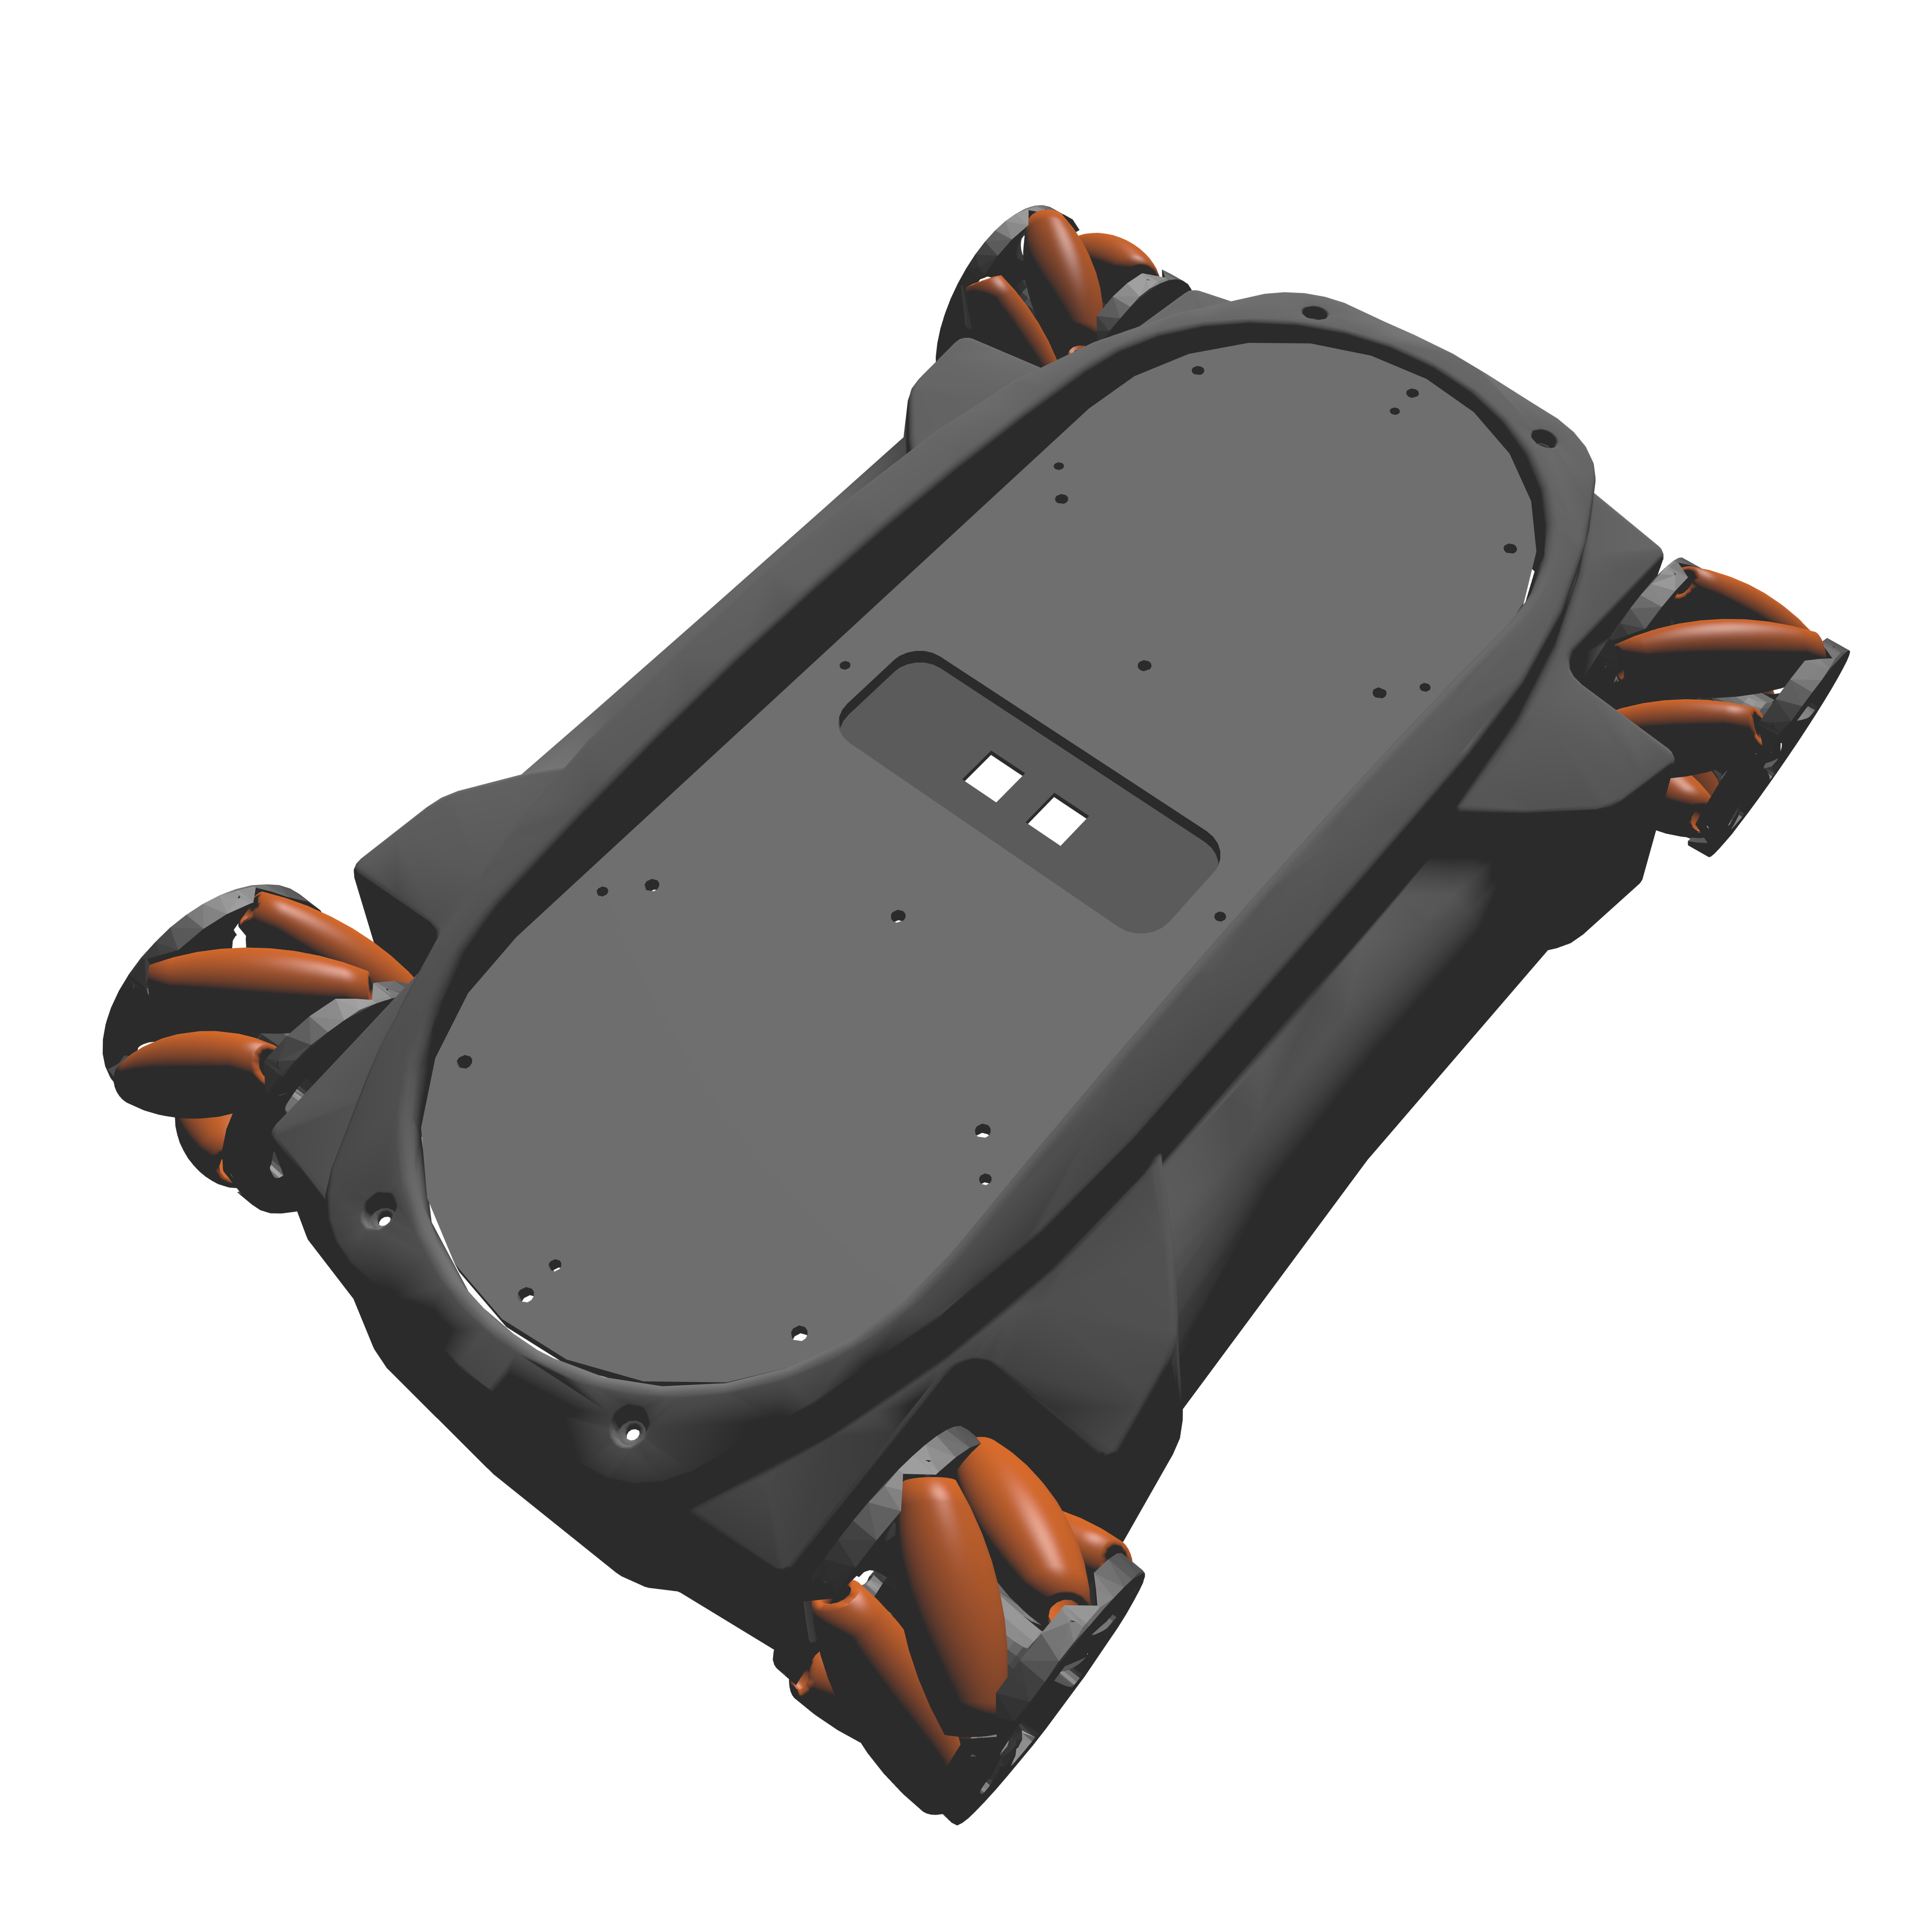
\includegraphics[width=0.5\textwidth]{graphics/kuka_youbot.png}
	\caption{Przykład innej platformy wielokierunkowej na podstawie fragmentu komercyjnego robota Kuka Youbot. 
	Należy zwrócić uwagę na charakterystyczne ustawienie kół, identyczne jak w opisywanej platformie \ref{fig:base_photo}.}
	\label{fig:kuka_youbot}
	\end{figure} 

	Odpowiedni obrót kół względem bazy, pozwala na jej ruch w dowolnym kierunku, niezależnym od kąta obrotu robota, patrz rysunek \ref{fig:mecanum_dirs}.
	Jest możliwe także obracać bazą, gdy ta porusza się w dowolnym kierunku, bądź stoi w miejscu.
	
	\begin{figure}[H]
	\centering
	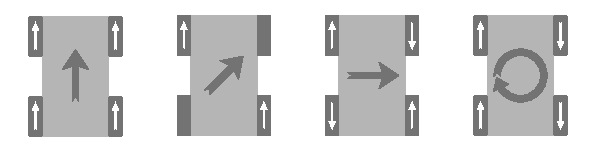
\includegraphics[width=0.8\textwidth]{graphics/mecanum_dirs.pdf}
	\caption{Podstawowe ruchy, jakie może wykonywać robot o napędzie wielokierunkowym.}
	\label{fig:mecanum_dirs}
	\end{figure} 
	
	Przykładowo, poruszając tylko przeciwległymi kołami po przekątnej, system będzie mógł poruszać po skosie, bez zmiany kąta obrotu.
	A jeśli do tego dodać obrót kół drugiej przekątnej, w odwrotnym kierunku, wtedy pojazd zacznie się poruszać w bok, pomimo faktu że koła nie są skrętne i 
	nie mogą ustawić się prosto do kierunku jazdy.
	Trasa po której porusza się robot, przy stałej prędkości kół, zawsze jest okręgiem, można uznać prostą za okrąg o nieskończonym promieniu, a punkt za okręg o zerowym.
	Wynika to z faktu, że każdy obiekt, który ma jednostajną prędkość i stały kierunek w lokalnym układzie współrzędnych, oraz prędkość kątową, będzie się poruszał po takiej krzywej.

	Podstawa ma za zadanie transportować robota manipulującego Velma, tworząc razem manipulator mobilny.
	Velma to wysoki i bardzo ciężki robot, wyposażony w dwa chwytaki na ramionach o wielu przegubach, patrz fotografia \ref{fig:velma}.
	Taka budowa wymaga szerokiej podstawy, aby zachować bezpieczną równowagę całości.
	Jeżdżąc na tej podstawie, robot może się przemieszczać i obracać w dowolnym kierunku, aby uzyskać lepszy dostęp do manipulowanych przedmiotów.
	Dodatkowe czujniki laserowe umieszczone tuż nad postawą odpowiadają za wykrywanie kolizji i lokalizację.

	\begin{figure}[H]
	\centering
	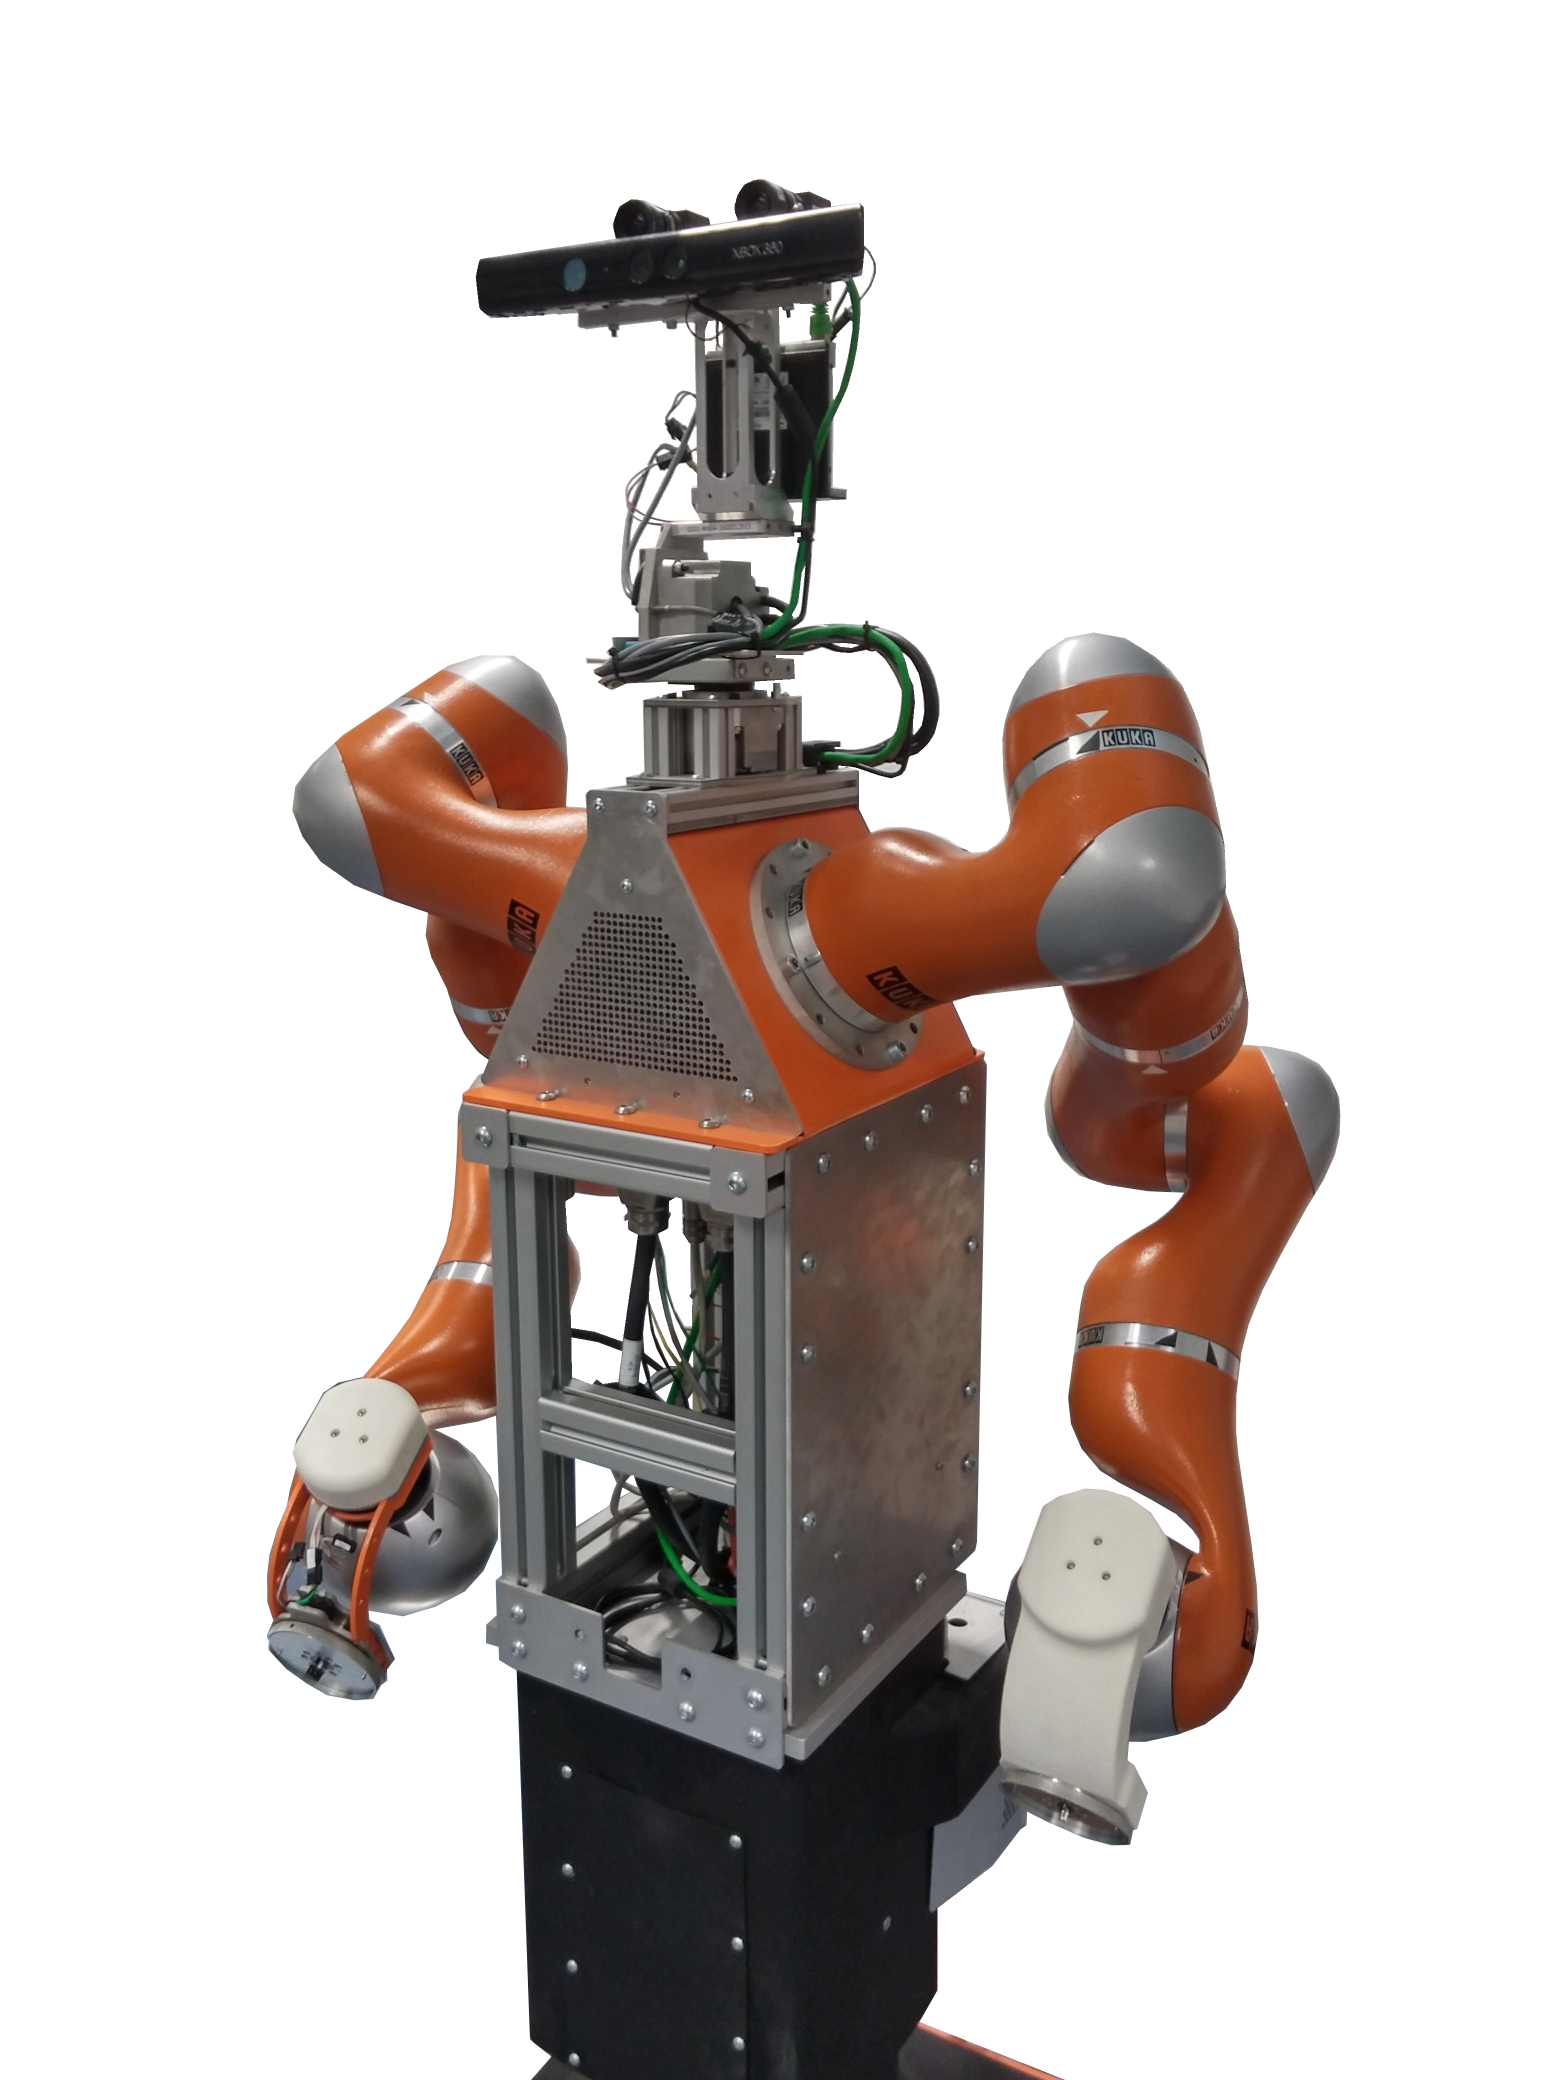
\includegraphics[width=0.5\textwidth]{graphics/velma.png}
	\caption{Robot manipulacyjny Velma.}
	\label{fig:velma}
	\end{figure} 

	Platforma jest niesymetrycznie podzielona na dwie niezależne części, przednią i tylną, w sposób pokazany na rysunku \ref{fig:base_top}.
	Przegub o jednym stopniu swobody (tzw. zawias) jest jedynym łącznikiem pomiędzy tymi dwoma fragmentami.
	Zadaniem tego przegubu jest zmniejszanie wpływu nierówności podłoża na ruch bazy, aby każde koło dociskało do podłoża z taką samą siłą, jak po drugiej stronie osi.
	Bez tego zawiasu nierówny teren uniemożliwiałby sprawne sterowanie platformą na skutek niedeterministycznego tarcia kół tej samej osi, powodując nieplanowany skręt.
	Niedeterministyczne tarcie kół jest niewykrywalne w bezpośredni sposób, więc należy je wyeliminować na przykład za pomocą takiego przegubu \cite{boringbot}.

	Platforma nie jest idealnym kwadratem, jest 4 cm różnicy między szerokością, a długością robota.
	Także środki kół nie są ustawione na wierzchołkach tej figury geometrycznej.
	Szerokość jest większa, co można zobaczyć porównując widok z prawej strony \ref{fig:base_side} z widokiem z tyłu \ref{fig:base_front}.
	Dokładne wymiary są podane na rysunku \ref{fig:base_dims} i tabeli \ref{tab:dims}.

	Platforma podatna jest na losowy ruch przy rozpoczynaniu jazdy i hamowaniu.
	Jest to spowodowane tym, że asymetria rolek będzie nadawać kołom różne siły oporu, a w związku z tym różne prędkości, co w efekcie może powodować niedeterministyczny ruch.
	Należy także wziąć tutaj pod uwagę inne cechy budowy kół, jak nierówne tarcie rolek o powierzchnię \cite{braking}.

	\begin{figure}[H]
	\centering
	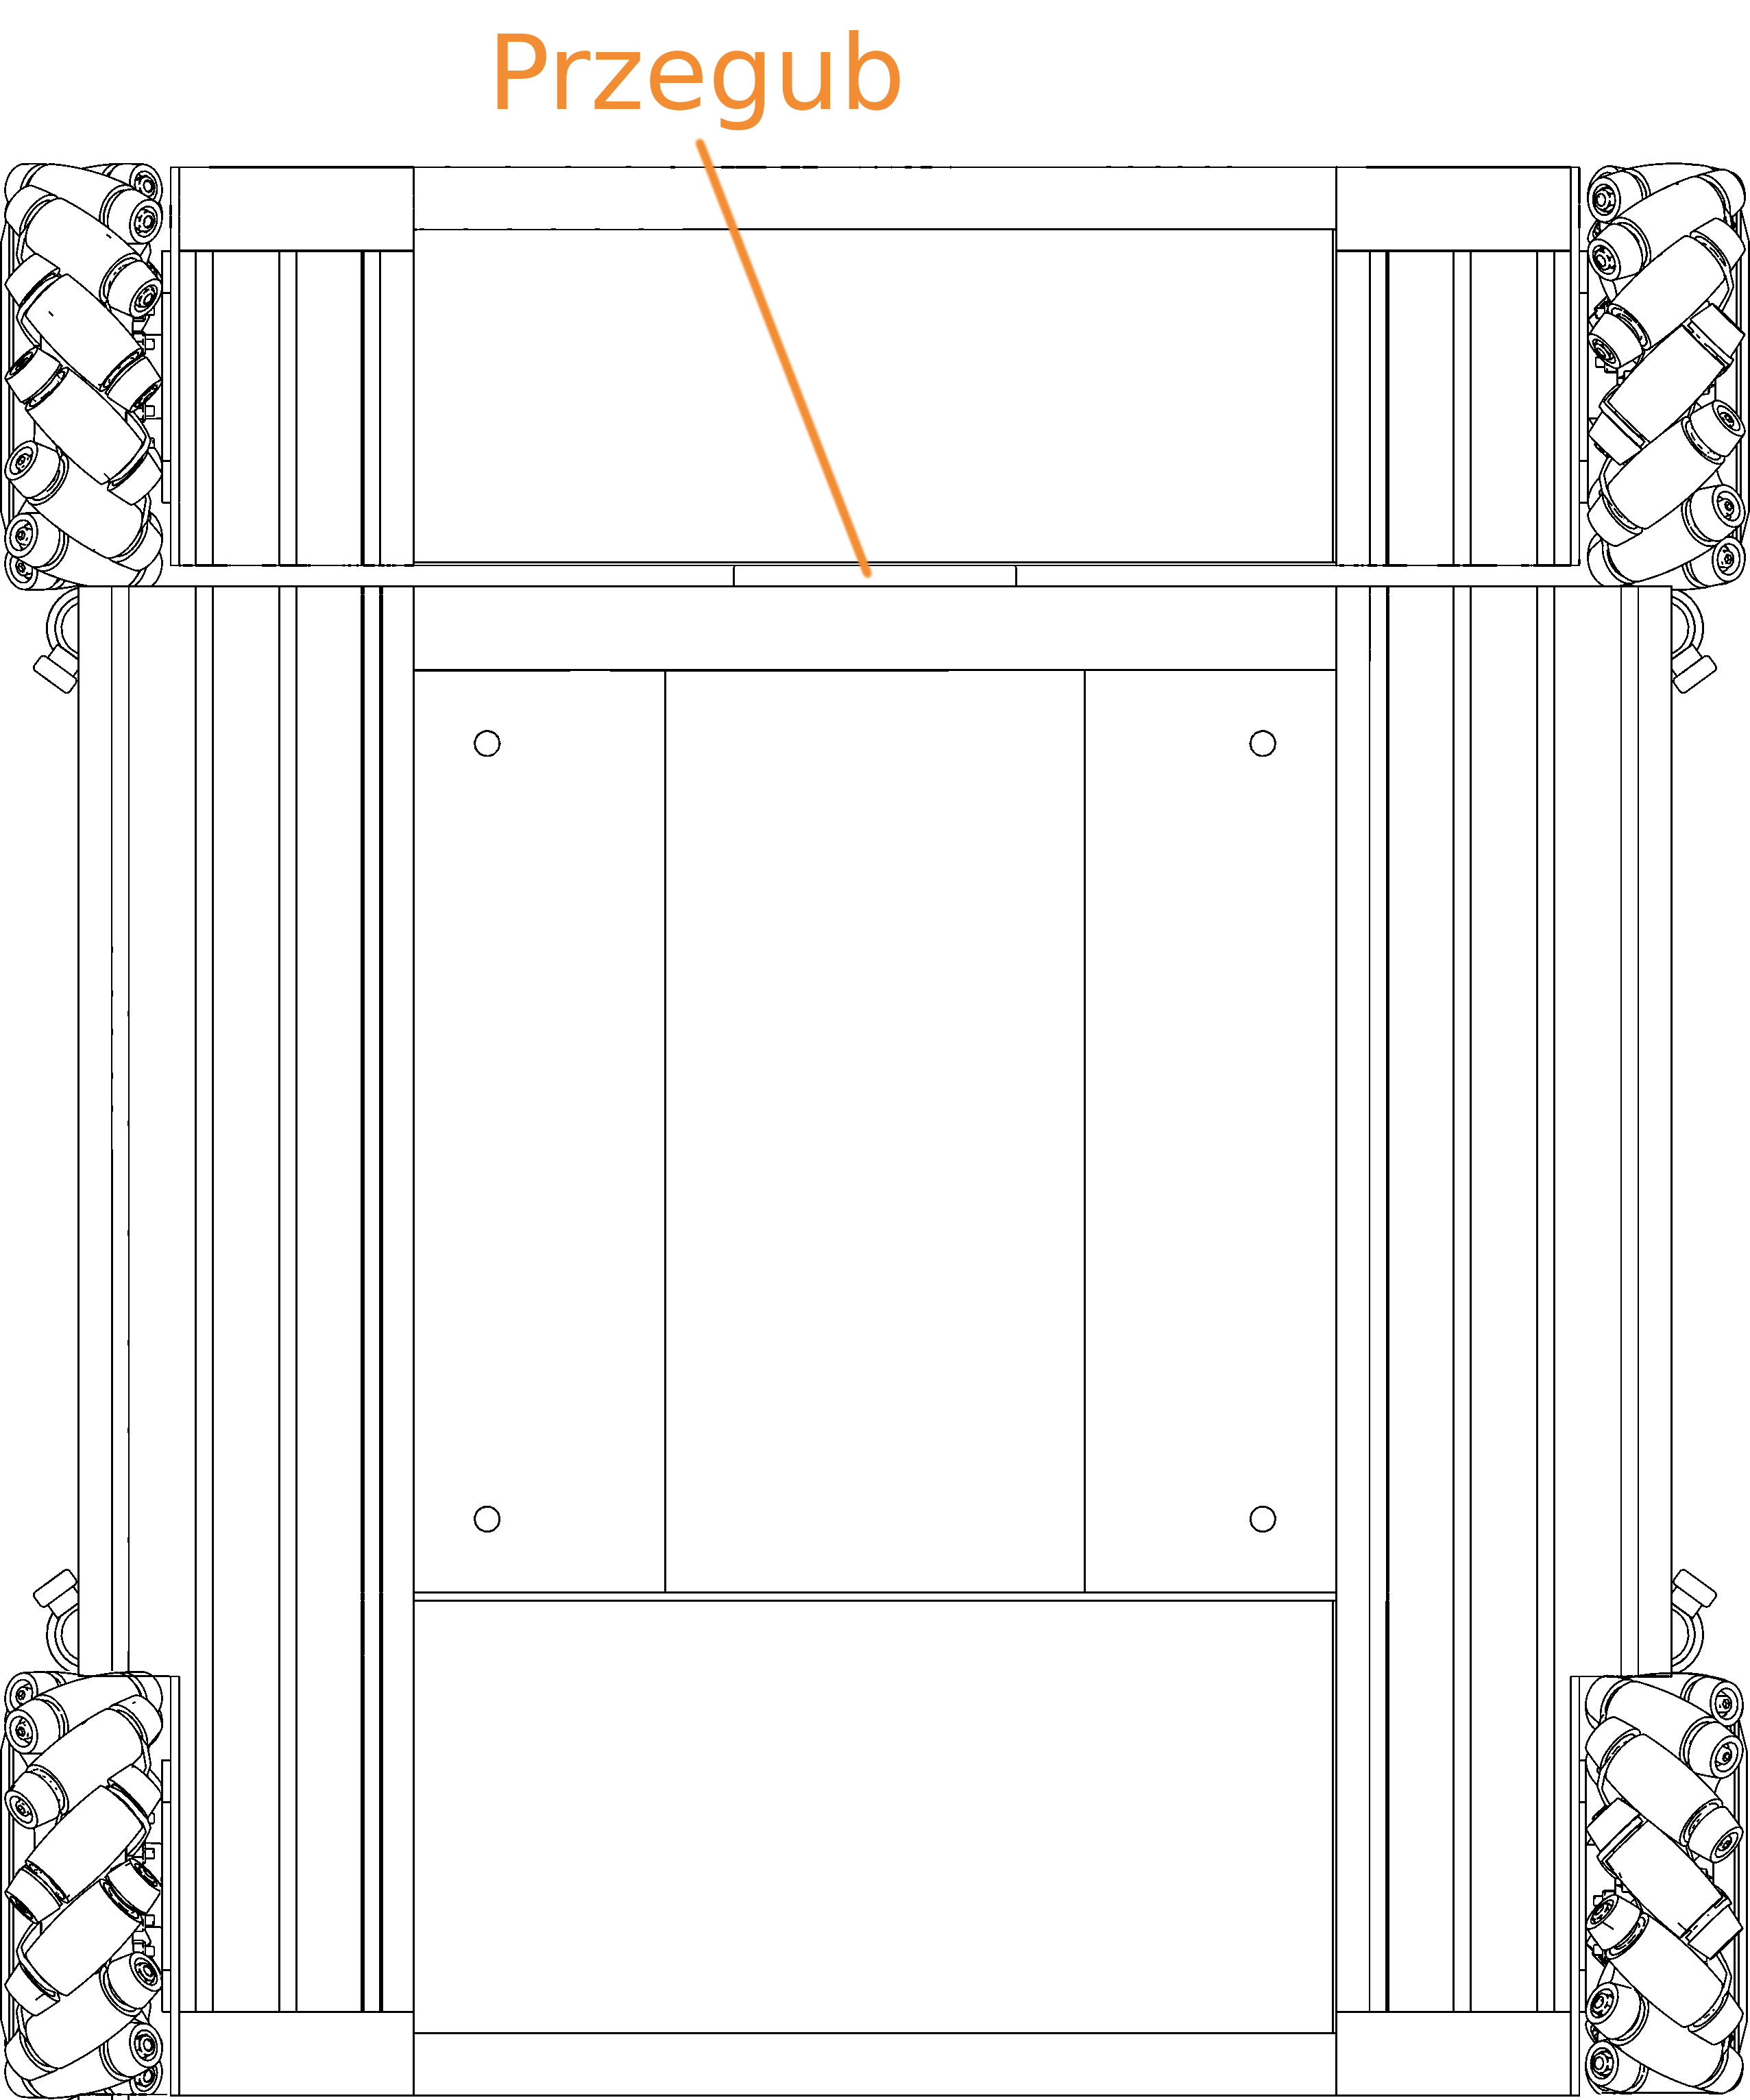
\includegraphics[width=0.5\textwidth]{graphics/base_top.png}
	\caption{Platforma mobilna --- widok od góry. Przegub zawiasowy łączy dwie części.}
	\label{fig:base_top}
	\end{figure} 

	\begin{figure}[H]
	\centering
	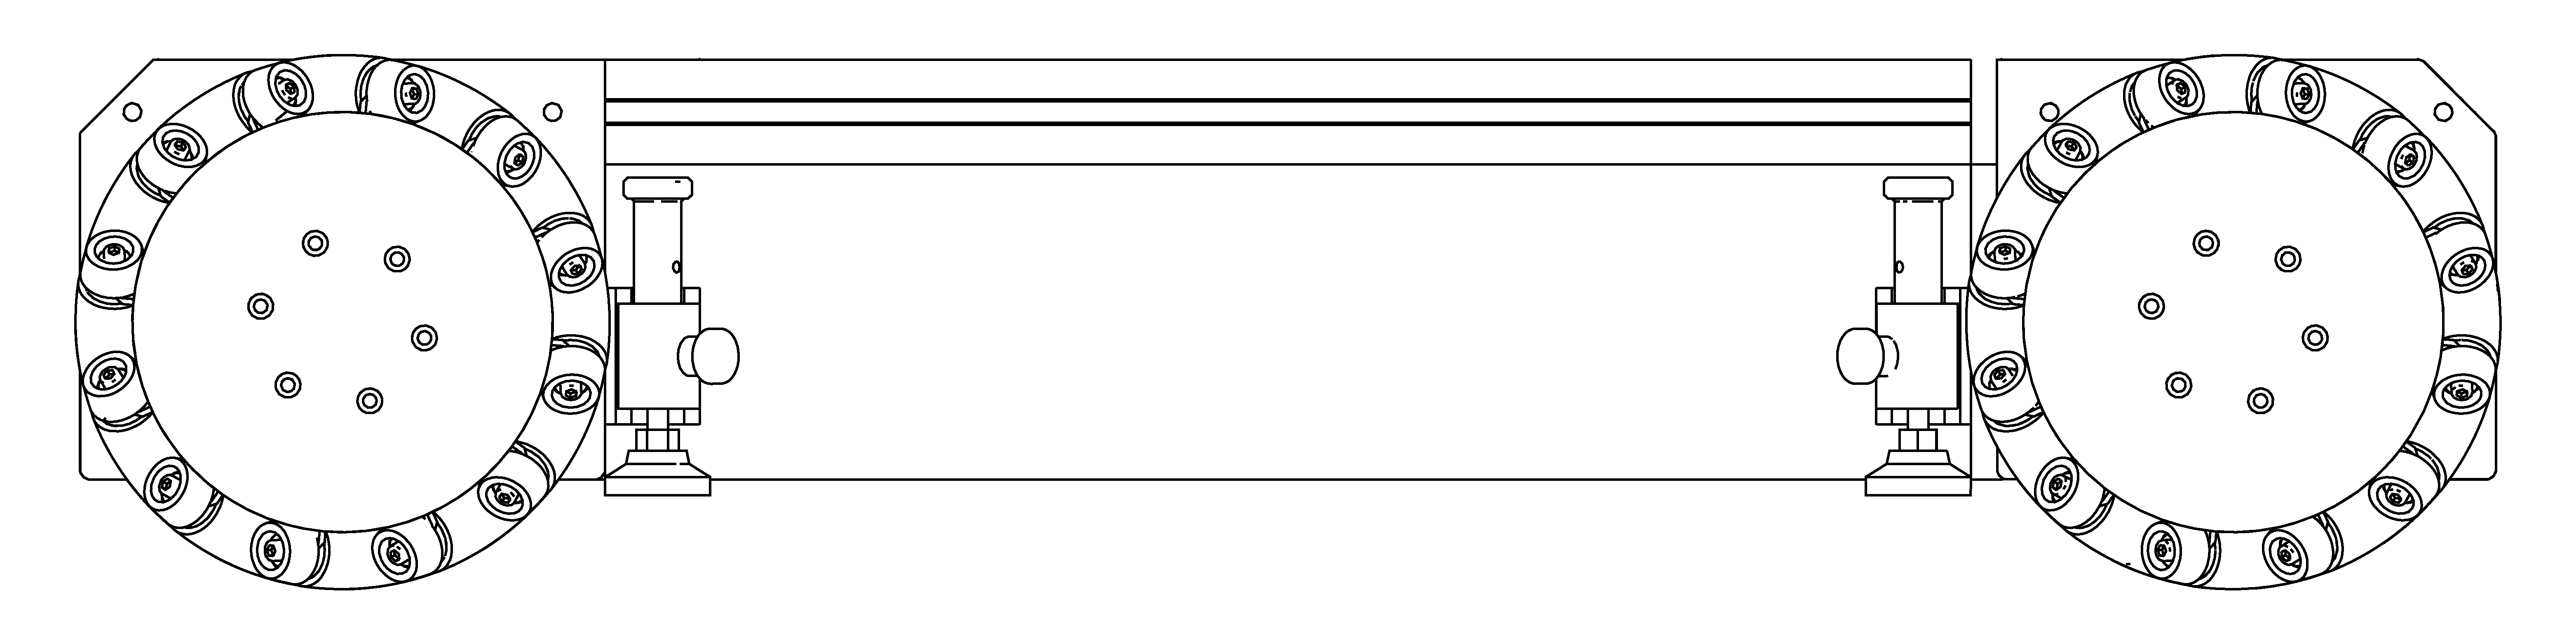
\includegraphics[width=0.5\textwidth]{graphics/base_side.pdf}
	\caption{Platforma mobilna --- widok z prawej strony.}
	\label{fig:base_side}
	\end{figure} 

	\begin{figure}[H]
	\centering
	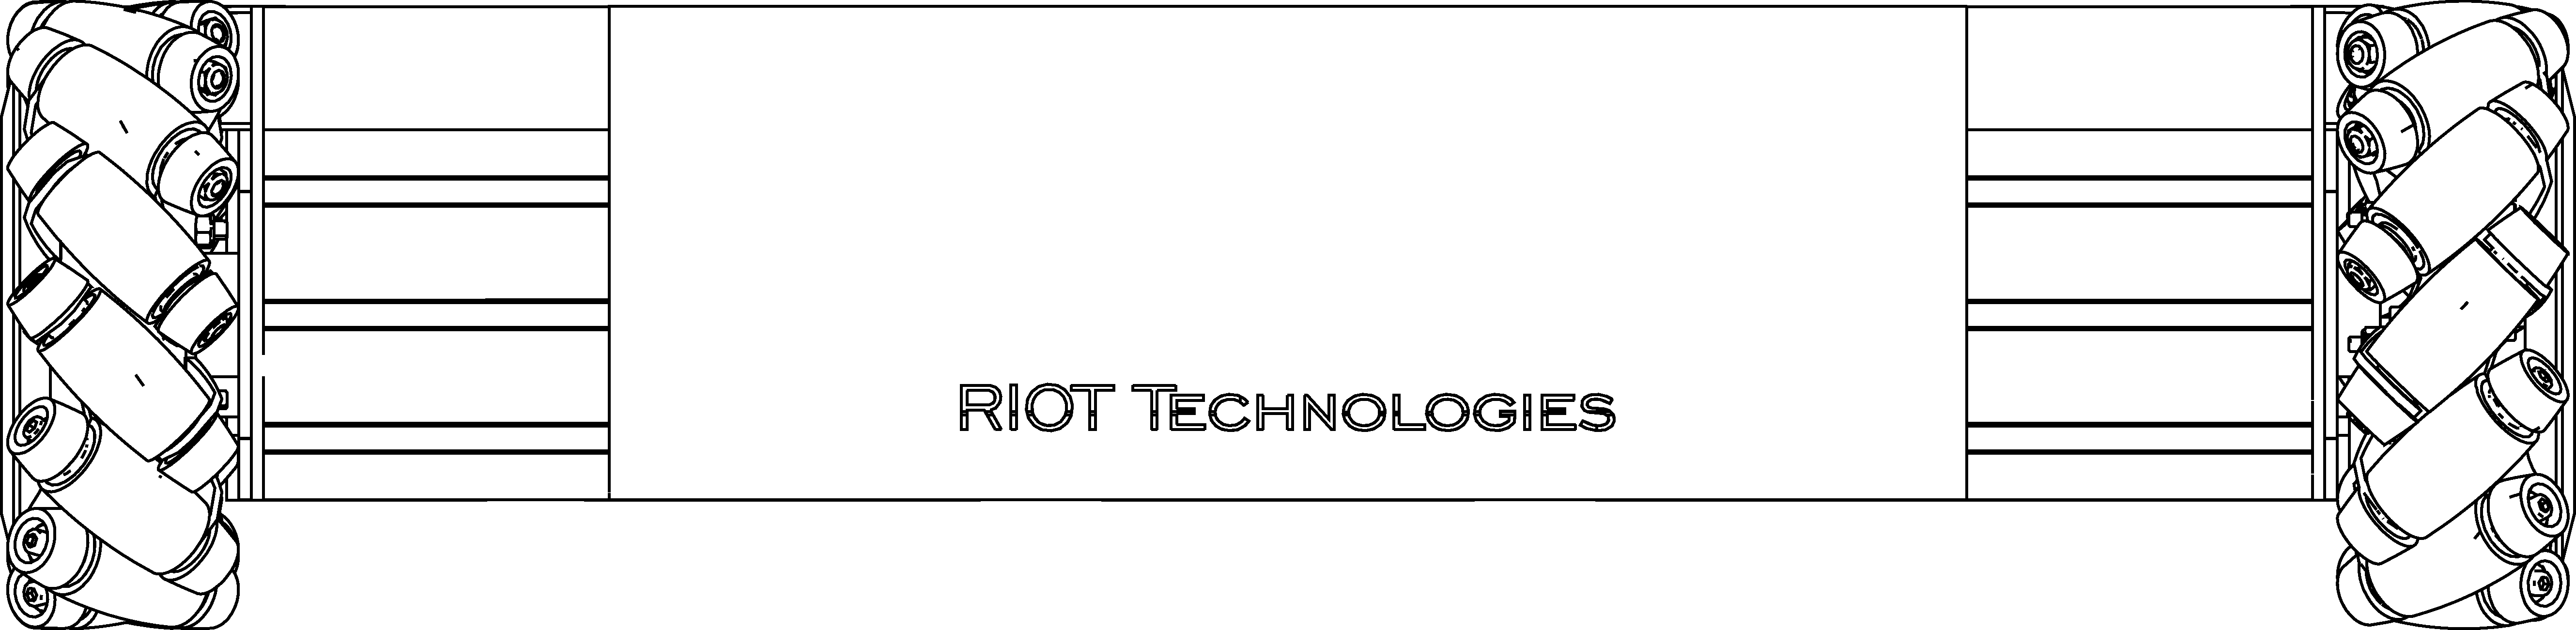
\includegraphics[width=0.5\textwidth]{graphics/base_front.pdf}
	\caption{Platforma mobilna --- widok z tyłu.}
	\label{fig:base_front}
	\end{figure} 

	Platforma posiada 3 stopnie swobody. 
	\begin{itemize}
		\item Ruch bez obrotu równolegle do osi X.
		\item Ruch bez obrotu równolegle do osi Y.
		\item Obrót w płaszczyźnie podłoża.
	\end{itemize}

\section{Koła szwedzkie}
	Koła szwedzkie, zwane także kołami Mecanum, to specjalne koła z dodatkowymi rolkami na obwodzie, ustawionymi pod kątem $45^\circ$ do osi koła.
	Rolki są pasywne i obracają się niezależnie od siebie. Każde koło ma 12 takich rolek, patrz rysunek \ref{fig:wheel}.
	W platformie ich osie ustawione są w ten sposób, że osie najwyższych, lub najniższych, rolek dwóch kół z tej samej strony robota przecinają się pod kątem prostym.
	Innymi słowy, robot ma identycznie ustawione koła na przeciwległych wierzchołkach, i razem ustawione są w kształt litery \emph{X} patrząc na nie z góry.
	Warto pamiętać, iż oś aktualnie dolnej rolki jest prostopadła do osi górnej rolki.

	Istnieje również odwrotna odmiana ustawienia kół, w której rolki tworzą literę \emph{O}, 
	czyli oś przednia jest zamieniona z tylną, lub jakby cała platforma była odwrócona do góry nogami.
	Ten drugi sposób także pozwala na ruch wielokierunkowy, ale nie jest tak często stosowany \cite{paletobot}.

	\begin{figure}[H]
	\centering
	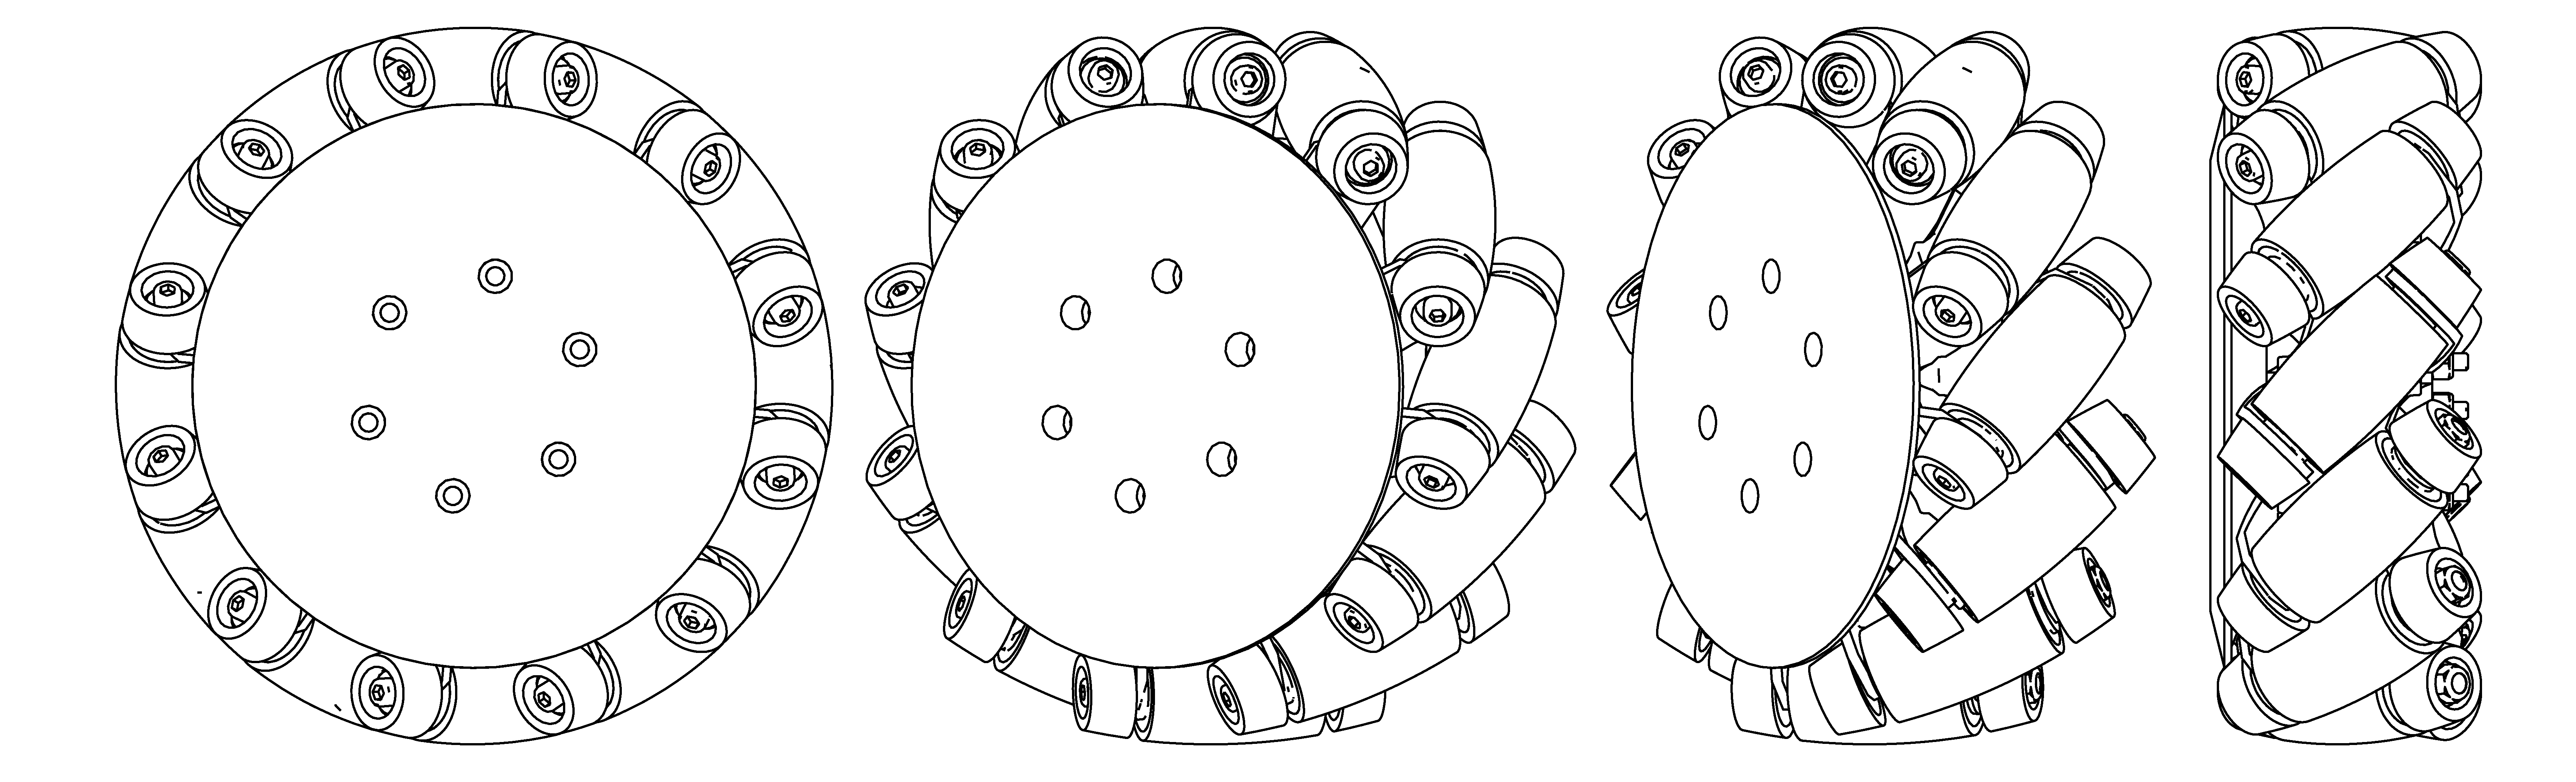
\includegraphics[width=\textwidth]{graphics/wheel.pdf}
	\caption{Widok 12 rolkowego koła szwedzkiego opisywanej platformy wielokierunkowej.}
	\label{fig:wheel}
	\end{figure} 

	Każde koło ma 3 stopnie swobody \cite{kinematic_modeling}, tak samo jak cała platforma.
	\begin{itemize}
		\item Obrót koła w osi.
		\item Rotacje pojedynczych rolek.
		\item Poślizg obrotowy w miejscu styku rolki z podłożem.
	\end{itemize}

	Na podstawie rysunku \ref{fig:wheel} widać, że krzywizna rolki jest tak ustawiona, aby punkt kontaktu rolki z podłożem w czasie obrotu płynnie przechodził na następną rolkę.
	Celem jest utrzymanie równej odległości osi od płaszczyzny podłoża.
	Nie powinno być efektu przeskoku z jednej rolki na drugą, gdyż to wprowadza nierówne tarcie, losowe poślizgi i nadmierne zużycie elementów wykonawczych.
	Kształt pojedynczej rolki zawiera się w paraboloidzie, wzory opisujące kształt rolki są złożone.
	Zazwyczaj przybliża się taką rolkę wycinkiem torusa, w celu uproszczenia produkcji \cite{rollers}.

	Istnieją także inne budowy kół, złożone z wielu małych rolek, tak aby w każdym momencie więcej jak jedna rolka dotykała podłoża.
	Można także złożyć kilka powyższych kół obok siebie w jedno koło.
	Przydatne jest to dla robotów transportujących duże masy, gdyż zmniejsza to obciążenie pojedynczych rolek.
	Niestety, taka budowa jest chroniona aktywnym patentem, więc pojedyncze koło, na które patent już wygasł, jest jedynym popularnie używanym \cite{paletobot}.

	Podstawowym problemem technologicznym koła jest nie tylko skomplikowana budowa, ale także ślizganie się rolek po powierzchni.
	Odległość osi od płaszczyzny nieznacznie zmienia się przy przenoszeniu ciężaru z rolki na rolkę, co przy dużych prędkościach powoduje drgania i jeszcze większe błędy pomiarów.
	Środkowy przegub zmniejsza ich przenoszenie na drugą część platformy.
	Poślizg kół powoduje, że enkodery nie mogą być jedynymi czujnikami służącymi do wyznaczania pozycji bazy, gdyż są zbyt mało dokładne \cite{heavy}.
	
	Dodano więc dwa czujniki laserowe, opisane dokładniej w sekcji \ref{sec:lidar}, aby program sterujący nie bazował jedynie na odometrii przy 
	wyznaczaniu sterowania.

	\subsection{Działanie platformy}
	Standardowe koło, używając tarcia, przekształca prędkość kątową na liniową w płaszczyźnie obrotu. 
	Specjalne koło Mecanum ma dodatkowy wektor, równoległy do osi obrotu, 
	zatem prędkość wypadkowa jest obrócona o 45° w stosunku do wektora prędkości standardowego koła, 
	zależnie od typu koła (prawoskrętne lub lewoskrętne) i kierunku obrotu.

	\begin{figure}[H]
	\centering
	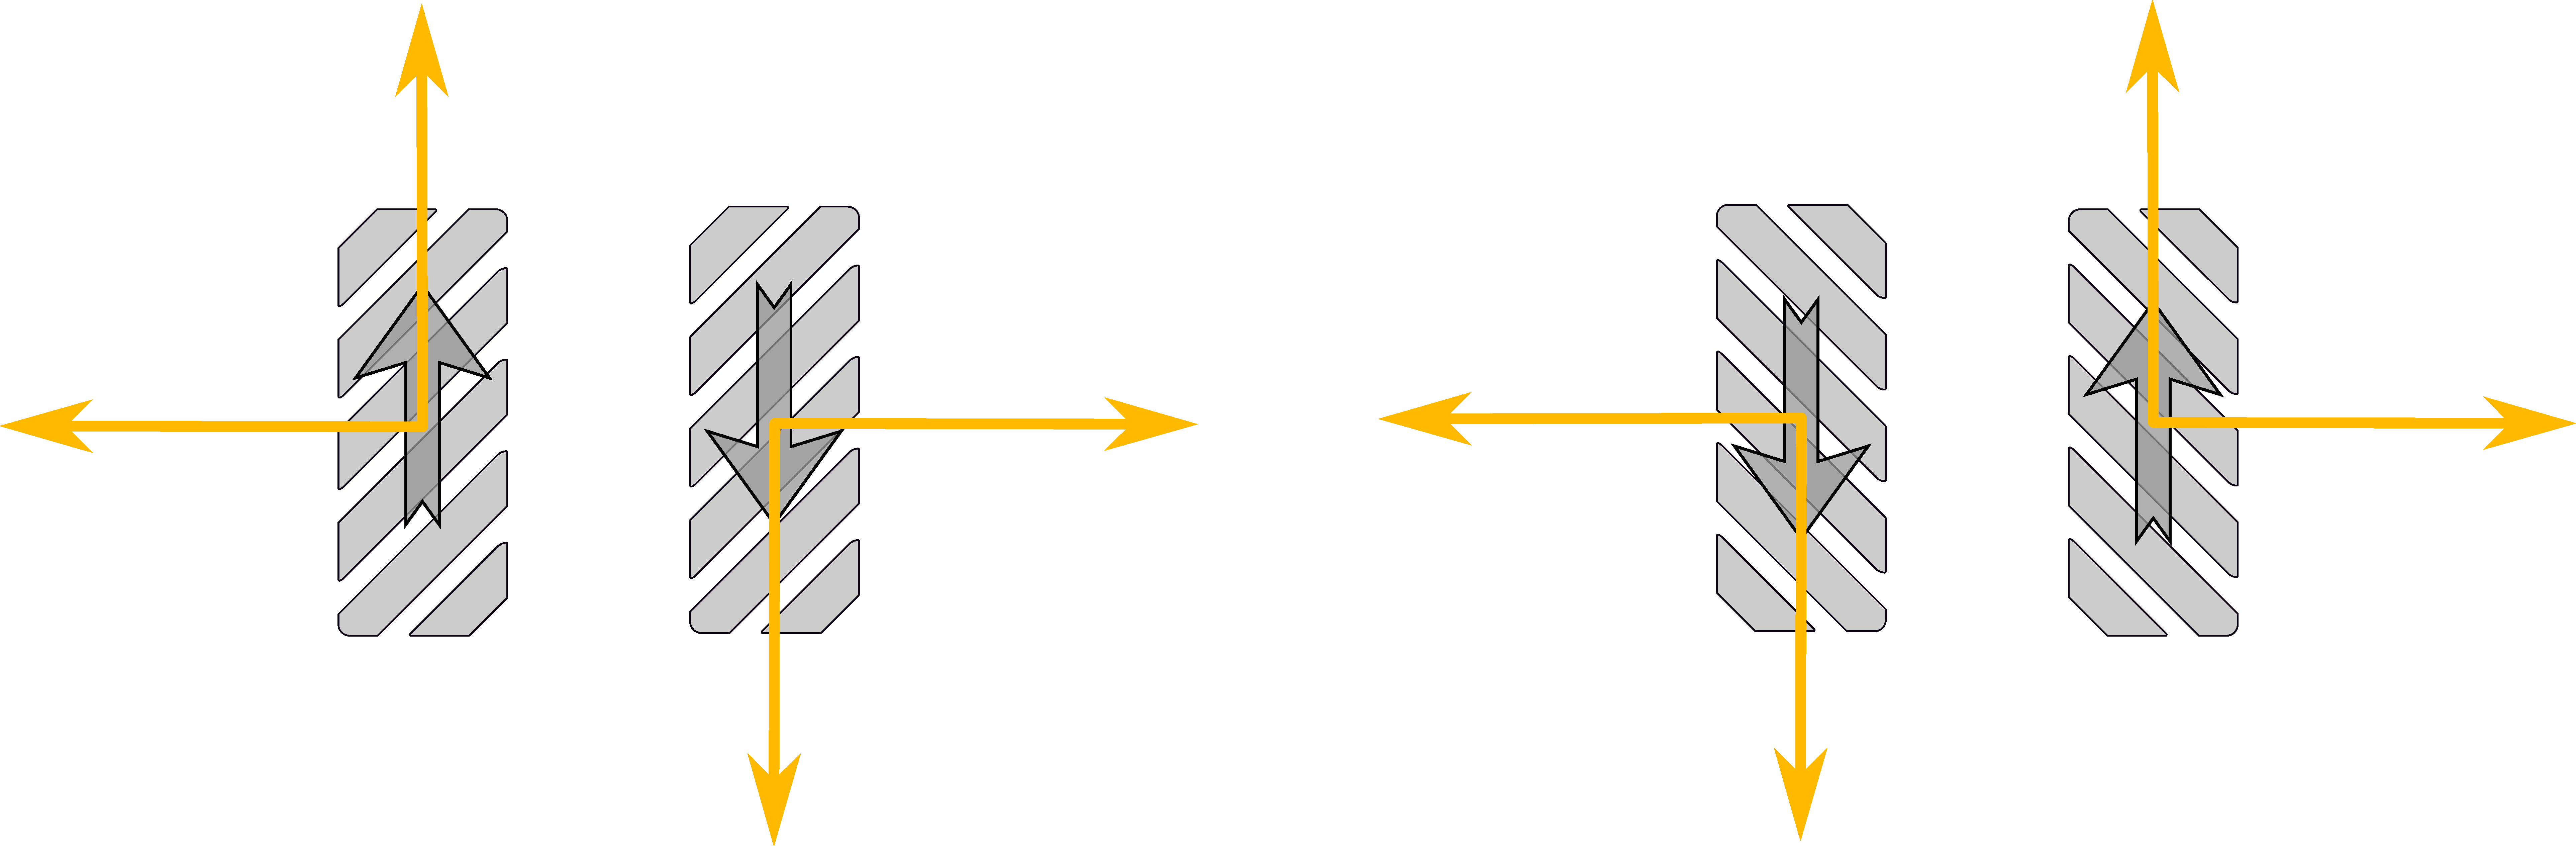
\includegraphics[width=\textwidth]{graphics/vectors.pdf}
	\caption{Wektory składowe i wypadkowe koła widzianego z góry.}
	\label{fig:wheel_vectors}
	\end{figure} 

	Ustawiając te koła w odpowiedni, opisany wcześniej na obrazku \ref{fig:base_top}, sposób, można wywołać odpowiednie znoszenie się składowych prędkości,
	a w efekcie pozwolić robotowi na poruszanie się w kierunkach nieosiągalnych dla pojazdów o standardowych kołach.
	Warto nałożyć te składowe na wcześniejszy rysunek \ref{fig:mecanum_dirs}, aby dokładniej zobaczyć, 
	dlaczego koła nadają platformie daną prędkość wypadkową przy odpowiednim obrocie kół.

	\begin{figure}[H]
	\centering
	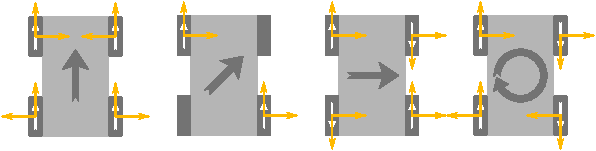
\includegraphics[width=\textwidth]{graphics/mecanum_dirs_vect.pdf}
	\caption{Ruchy platformy widzianej z góry, z nałożonymi składowymi wektorów prędkości. Ciemniejszym kolorem zaznaczono znoszące się składowe.}
	\label{fig:mecanum_dirs_vect}
	\end{figure} 

	Warto rozpatrzyć każdy przypadek.
	\begin{enumerate}
		\item Wektory o kierunku prostopadłym do pionowej płaszczyzny symetrii urządzenia znoszą się, pomimo że mają przeciwne zwroty na przedniej i tylnej parze kół.
		Pozostają jedynie składowe równoległe do płaszczyzny symetrii, które powodują prostoliniowy ruch naprzód.
		\item Dwa koła nie obracają się. Nie jest to ruch pasywny, gdyż taki wprowadzałby nieprzewidywane poślizgi, a aktywne hamowanie.
		Wektory się nie znoszą i platforma wykonuje ruch pod kątem 45° do płaszczyzny symetrii.
		\item Ruch podobny jest do przypadku 1. Tutaj również wektory znoszą się parami, jednak tym razem na prawych kołach i lewych. 
		Różnica ruchów polega na większej prędkości obrotu pojedynczych rolek wokół ich osi.
		\item Prędkość kątowa powstaje, gdy wypadkowa kół po jednej stronie platformy znosi się z wypadkową po drugiej stronie.
	\end{enumerate}

	Warto nadmienić, że gdy wypadkowy wektor prędkości koła jest prostopadły do osi koła, to jest gdy
	koło porusza się zgodnie z kierunkiem obrotu, w idealnym przypadku rolki nie obracają się.
	Inaczej mówiąc, rolka będzie się obracać tym mocniej, im bardziej ruch koła wymuszany jest równolegle do osi koła, 
	czy to na skutek znoszenia się wektorów, czy oporu przeszkody.
	
	Przykładowo, przy ruchu naprzód rolki koła się nie obracają, lecz przy ruchu w bok biorą aktywny udział.
	Ma to wpływ na zużywanie się tych elementów, nie tylko z punktu widzenia ilości obrotów danej rolki na pokonanym dystansie, 
	ale także sposobu w jaki wymuszany jest jej ruch.
	Rolki robota przy jeździe zawsze obracają się szarpanym ruchem w obie strony, ze względu na poślizgi od innych kół, 
	niejednostajne tarcie piast wszystkich rolek, czy różnice terenu. 
	Zatem przejazd przykładowego odcinka, przy platformie ustawionej przodem do kierunku jazdy, lub bokiem, będzie w różnym stopniu i w różny sposób zużywał elementy wykonawcze robota.
	To, jaki styl jazdy opłaca się zastosować, aby zminimalizować zużywanie się elementów jest dużą, odrębną dziedziną nauki.
	Odpowiednio skomplikowany algorytm sterowania może brać pod uwagę to zachowanie się tych elementów składowych.

\section{Czujnik laserowy}
	\label{sec:lidar}
	Program sterujący platformą nie jest w stanie dokładnie określić pozycji robota, bazując jedynie na odometrii.
	Potrzebny jest zatem czujnik laserowy.
	Platforma wyposażona jest w dwa, dwuwymiarowe czujniki typu LiDAR firmy SICK.
	LiDAR to zbitek wyrazów \emph{light} i \emph{radar}, chociaż skrót może być rozwinięty w różne słowa.

	\begin{figure}[H]
	\centering
	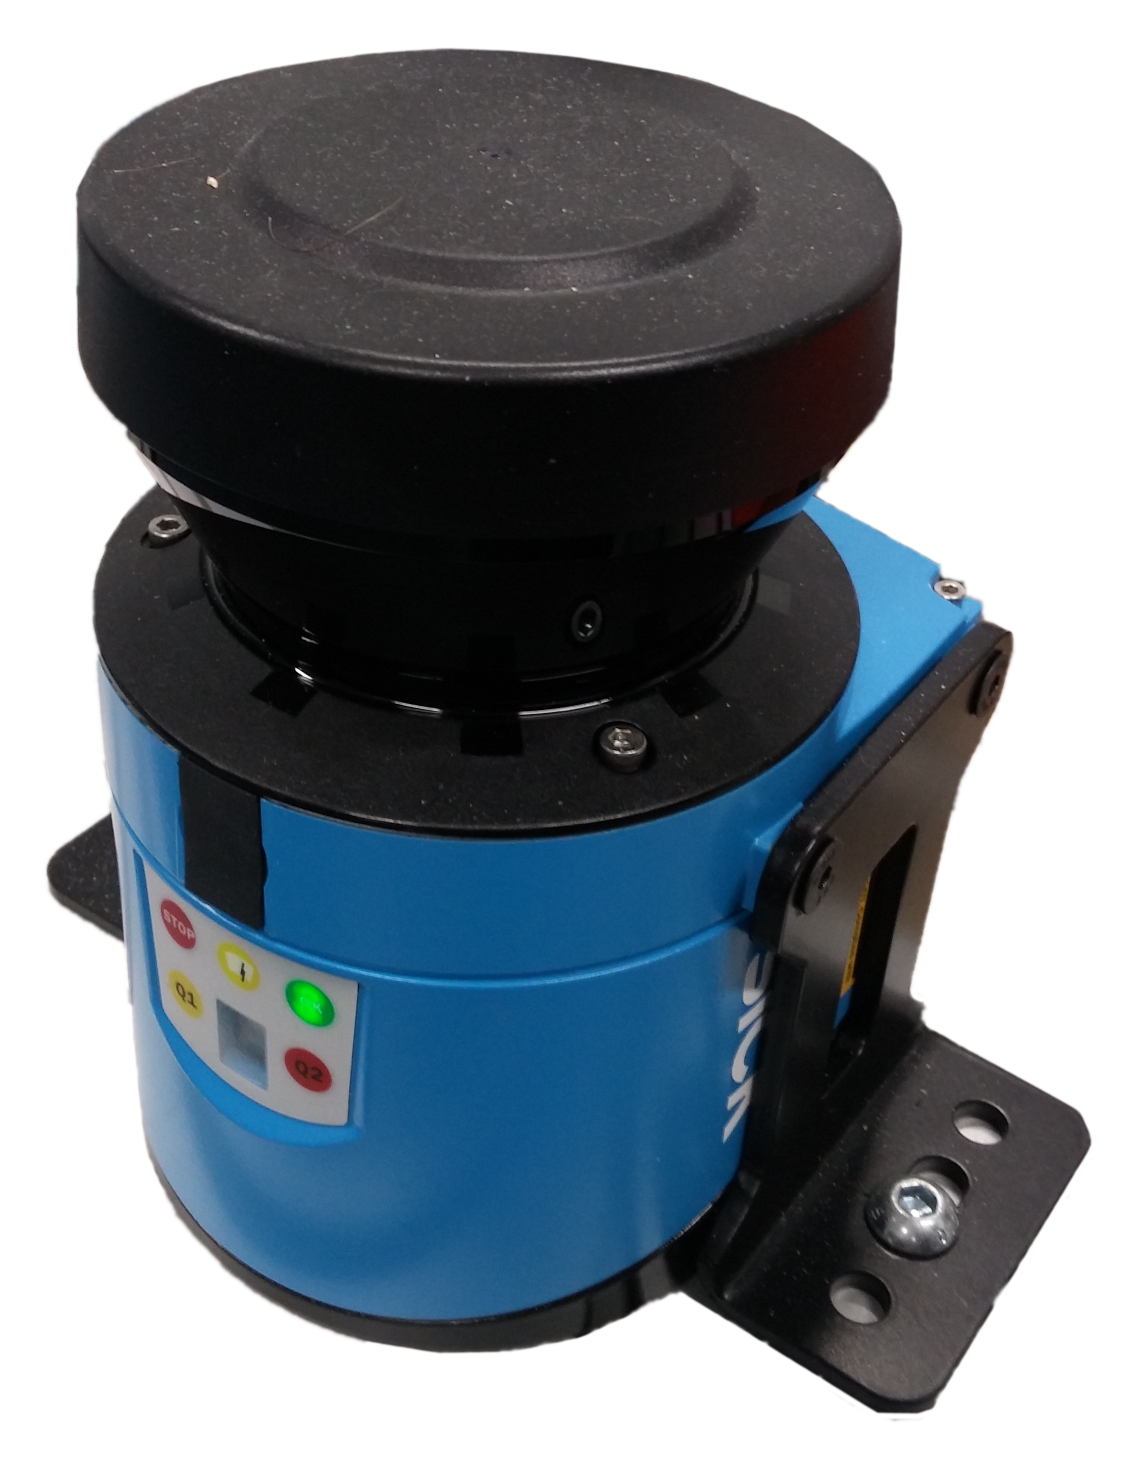
\includegraphics[width=0.5\textwidth]{graphics/sensor.png}
	\caption{Czujnik laserowy SICK LMS100-10000.}
	\label{fig:sensor}
	\end{figure} 

	\subsection{Zasada działania}
	Wszystkie czujniki tego typu mają bardzo podobną zasadę działania.
	W środku urządzenia znajduje się obrotowe lusterko, zwrócone pod kątem 45° do osi obrotu.
	Równolegle do osi jego obrotu znajduje się laser, który emituje pulsacyjną wiązkę podczerwonego promienia co pewien okres czasu.
	Aktualna pozycja lusterka jest wykrywana przez enkoder.
	Obok lasera jest czujnik, który bada wysłane przez laser, odbite od lusterka, obiektu i ponownie lusterka, światło.

	Na koniec, algorytm we wbudowanym mikrokontrolerze ustala kąt i odległość czujnika od wykrytego obiektu.
	Odpowiada także za usunięcie szumu i ewentualnych odbić promienia.
	Komunikacja z urządzeniem odbywa się za pomocą różnych interfejsów sieciowych, zazwyczaj w architekturze typu master-slave.
	
	Skośna szyba, będąca wycinkiem powierzchni stożka, zabezpiecza wnętrze przed zanieczyszczeniami, jej kształt niweluje ewentualne odbicia lasera, spowodowane jej istnieniem.
	W niektórych czujnikach montuje się także szereg dodatkowych diod podczerwieni na obrębie szyby, skierowanych w górę, oraz czujniki/reflektory z drugiej strony.
	Pozwala to na wykrycie stopnia zanieczyszczenia szyby, aby powiadomić użytkownika o potrzebie wyczyszczenia urządzenia.

	\subsection{Komunikacja}
	Wysyłając do czujnika odpowiedni ciąg bajtów, można ustawić jego tryb działania, odpytać o zebrane dane, czy wykryć konfigurację i stan.

	W przypadku naszej platformy, komunikacja odbywa się poprzez interfejs Ethernetowy.
	Program komunikujący się bezpośrednio z urządzeniem zwraca pakiety zawierające pomiary z ostatniego obrotu czujnika, oraz dodatkowe dane 
	opisujące sam pomiar, takie jak czas, początkowy kąt pomiaru, tryb itp.
	Dokładne dane i cechy czujnika dostępne są na stronie producenta \cite{sick_website}.

	Urządzenie wspiera uwierzytelnianie przez hasło, wgrywanie nowego oprogramowania,
	ustawienia czasu, oraz zmianę różnych parametrów działania.

	\subsection{Podstawowe cechy}
	Czujnik składa się z dwóch części, głównego trzonu, oraz nakładki.
	Połączenie tych elementów powoduje, że jego zakres pomiaru posiada martwy kąt.
	Przedstawia to dobrze grafika producenta.
	\begin{figure}[H]
	\centering
	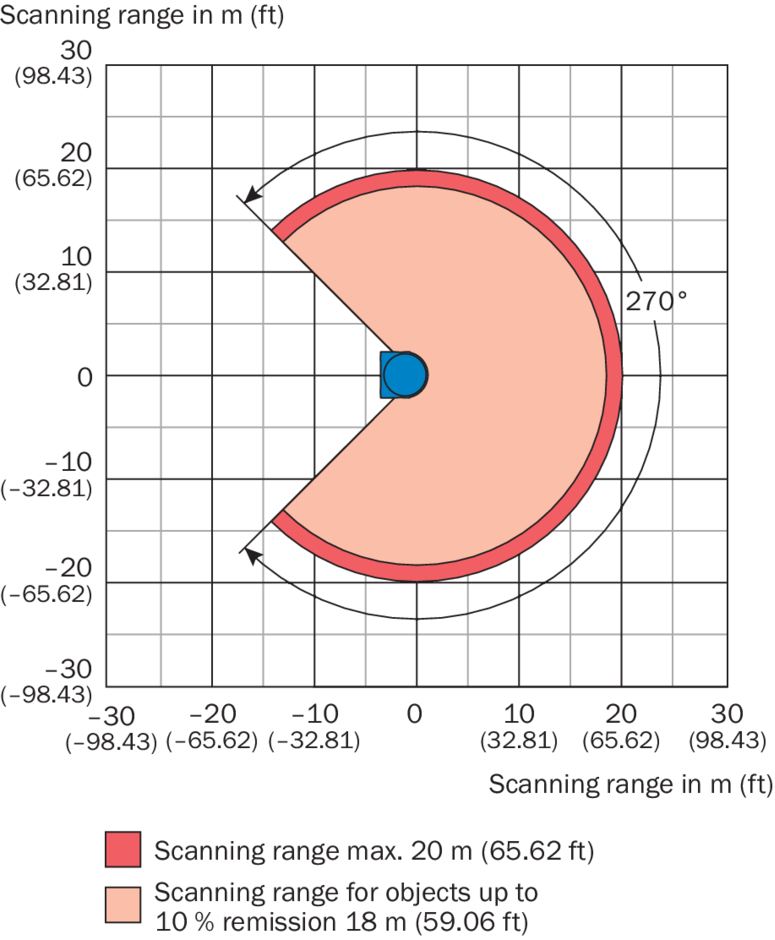
\includegraphics[width=0.6\textwidth]{graphics/sick.png}
	\caption{Wykres producenta dotyczący zasięgu czujnika.}
	\label{fig:lidar}
	\end{figure} 
	
	\begin{table}
	\centering
	\begin{tabular}{l r}
	Cecha & Wartość \\
	\hline
	Kąt pracy & 270\textdegree \\
	Długość fali światła lasera & 905 nm (podczerwień) \\
	Częstotliwości skanowania & 25 Hz / 50 Hz \\
	Maksymalna odległość obiektu & $\approx$ 20 m \\
	Rozdzielczość kątowa & $0,25 \degree$ / $0,5 \degree $ \\
	Systematyczny błąd pomiarowy & $\pm 0,03$ m \\
	Przypadkowy błąd odległości & $0,012$ m \\
	\end{tabular}
	\caption{Podstawowe cechy czujnika laserowego.}
	\label{tab:lidar}
	\end{table}
	Urządzenie jest w stanie komunikować się za pomocą portu szeregowego RS-232, połączenia Ethernetowego i sieci CAN.

\section{Składniki systemu}
	Środowisko symulacyjne składa się z kilku odrębnych modułów, które komunikują się ze sobą poprzez specjalne interfejsy, wykorzystujące kolejki wiadomości.
	Taka implementacja komunikacji pozwala zmieniać i reimplementować poszczególne elementy i używać różnych języków programowania, 
	zachowując jednolitą komunikację między składnikami i nie tracąc na kompatybilności między komponentami.
	Możliwe jest także przesyłanie wiadomości przez sieć, co pozwala na rozproszenie systemu.

	%TODO Zmienić na Tikz
	\begin{figure}[H]
	\centering
	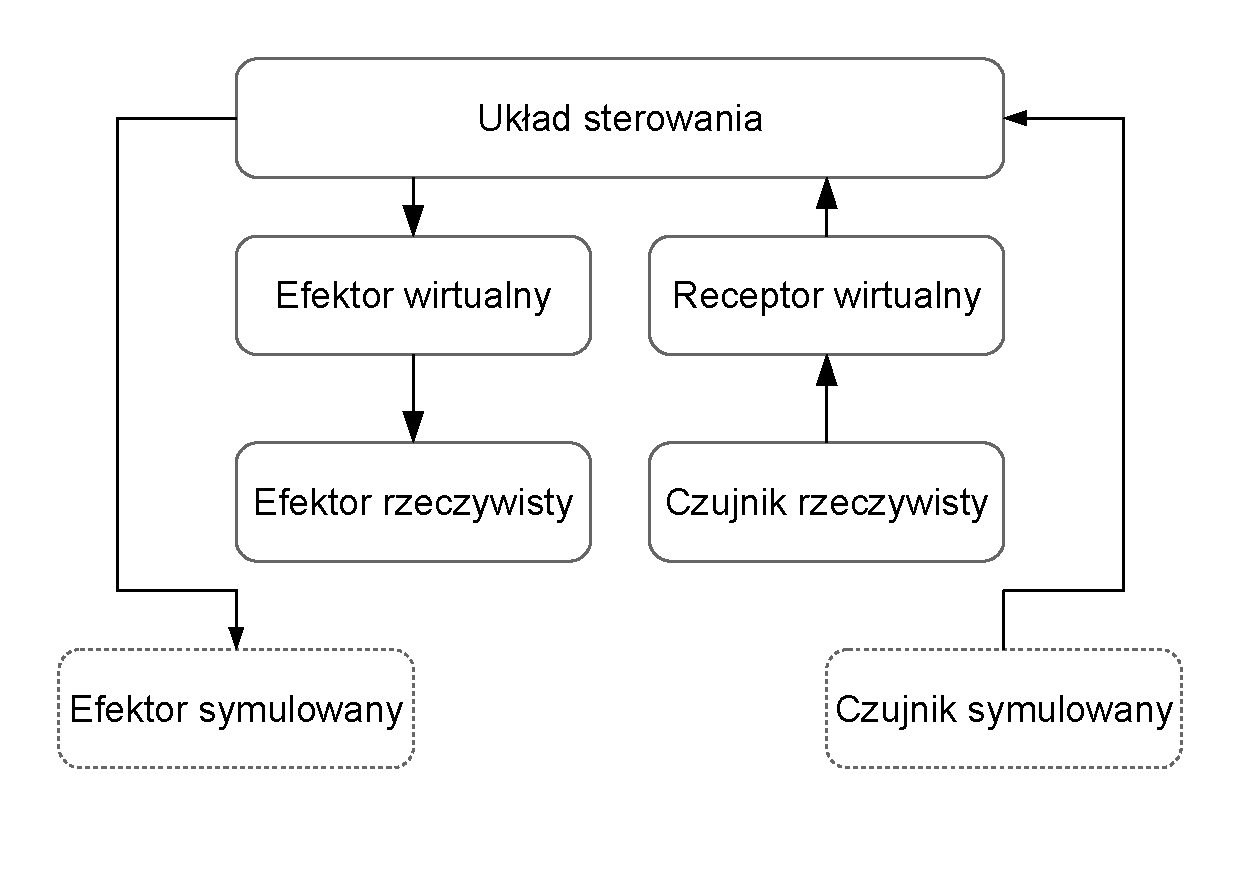
\includegraphics[width=0.8\textwidth]{graphics/agent.pdf}
	\caption{Struktura agenta upostaciowionego.}
	\label{fig:agent}
	\end{figure} 

	Można to przedstawić za pomocą zapisu agentowego, rysunek \ref{fig:agent}.
	Agent upostaciowiony składa się z kilku modułów, komunikujących się ze sobą za pomocą różnych interfejsów.

	Nadrzędnym modułem jest układ sterowania, który na podstawie odczytów z czujników generuje sterowanie dla efektorów.
	Ważne jest, aby komunikacja z rzeczywistymi urządzeniami była identyczna, jak z ich modelami, dzięki czemu taki system będzie przenośny i niezależny od implementacji modelu.

	Efektor rzeczywisty, na przykład serwomotor, jest sterowany za pomocą efektora wirtualnego, który zamienia wyjście układu sterowania na sygnały sterujące dla silnika napędowego.
	Przykładowo, zmienia odebraną liczbę, oznaczającą zadaną prędkość, na odpowiednie napięcie na wyjściu układu sterującego.

	Zamodelowany efektor symulowany również przyjmuje te same sygnały do układy sterowania, co efektor rzeczywisty, 
	lecz nie zamienia ich na sygnały sterujące, a wywołuje odpowiednie funkcje maszyny symulacyjnej, nadające siły i prędkości obiektom w przestrzeni wirtualnej.

	Receptor wirtualny pobiera surowe dane z czujnika, przekształca na odpowiedni format, usuwa błędy i szum tak, aby program sterujący mógł wykorzystać te dane w prosty sposób. 
	Doskonałym przykładem jest tutaj urządzenie Kinect (widoczne na robocie Velma na fotografii \ref{fig:velma}), w którym to zachodzi odczytanie obrazu z kilku kamer.
	Następnie obraz przesyłany jest do komputera, w którym sterowniki interpretują dane, usuwając błędy, tworzą mapę głębokości, wykrywają szkielety i sylwetki osób.
	Te dane mogą być wykorzystane łatwo w grach i programach sterujących.

	Modelowanie receptora, tak jak w przypadku efektora, polega na wygenerowaniu odpowiednich danych, używając odpowiednich funkcji w przestrzeni wirtualnej.
	Mogą one polegać na emitowaniu półprostych, symulujących laser, lub wręcz renderowaniu obiektów, aby uzyskać obraz z wirtualnej kamery.
	Receptor symulowany ma pełną wiedzę o symulowanym świecie, dokładne pozycje i prędkości wszystkich obiektów, dane o kolizjach itp. 
	Pozwala to na łatwe symulowanie receptorów nie mogących mieć odwzorowania w rzeczywistości, co przydatne jest w pierwszych stadiach testowania i wyznaczaniu statystyk.
	Takim przykładem jest model czujnika dokładnej pozycji, rotacji i prędkości w kartezjańskim układzie współrzędnych. 
	Czujniki typu GPS, lub żyroskopy nie generują tak dokładnych pomiarów.

	\subsection{Model 3D}
	Model 3D bazy mobilnej, opisany równaniami matematycznymi, powinien mieć zachowanie zbliżone do oryginału, najbardziej jak to tylko możliwe.
	Musi uwzględniać masy i momenty bezwładności elementów składowych, a także wszystkie tarcia.
	Model obejmuje więzy na ruchome elementy, takie jak koła i rolki, aby umożliwić symulację przegubów.

	Model składa się z elementów, odwzorowujących rzeczywiste części składowe bazy mobilnej.
	Elementy posiadają takie cechy, jak pozycja w modelu, masa, moment bezwładności, kształt, materiał fizyczny i wygląd.
	Dodatkowo należy uwzględnić wszystkie więzy, w postaci symulowanych przegubów.
	W przypadku tej bazy istnieje typ więzów o jednym stopniu swobody (zawias), używany przy połączeniu przedniej i tylnej części platformy, oraz 
	jako piasty kół i rolek. Można także uznać, że więzy bez stopni swobody używane są do trwałego połączenia czujników z platformą i transportowanym robotem.
	Więzy mogą oddziaływać siłą na elementy do których są podłączone, symulując silniki.

	Elementy składowe i symulowane przeguby oddziałują bezpośrednio z maszyną do symulacji fizycznej. 
	To kształt, masy i momenty bezwładności brył są argumentami funkcji liczących.
	Maszyna symulacyjna oblicza odpowiednie prędkości i nadaje je podanym obiektom w podobny sposób, jak ma to miejsce w rzeczywistości.

	Do modelu doczepia się wirtualne czujniki, generujące odpowiednie dane na podstawie symulacji i rozkładu losowego.
	Nie są to pełne dane o stanie modelu, jakie posiada maszyna do symulacji, gdyż czujniki fizyczne również nigdy nie mają pełnej informacji o stanie urządzenia.
	Należy dodać losowy szum i błędy, aby przybliżyć ich zachowanie do rzeczywistych czujników.

	Dla ozdoby można wykorzystać istniejący model CAD do stworzenia siatki trójwymiarowej i nadania symulowanemu obiektowi wyglądu zbliżonego do fizycznego robota.

	\subsection{Sterownik silników}
	Program sterujący generuje abstrakcyjne dane, na przykład liczbę zmiennoprzecinkową, zapisaną binarnie.
	Przykładowy silnik fizyczny nie jest w stanie działać na ich podstawie, sam silnik do pracy potrzebuje odpowiedniego napięcia na wejściu,
	ale interfejs serwomotoru na przykład przyjmuje bardziej abstrakcyjne dane.
	Do tłumaczenia jednych danych na drugie, potrzebny jest sterownik niskopoziomowy.
	Najczęściej implementowany jest w formie mikrokontrolera, lub podobnego systemu wbudowanego.

	Jego zadanie to odczytanie danych podanych przez program sterujący i na przykład generowanie na ich podstawie odpowiedniej fali PWC, lub obsługa przetwornika cyfrowo-analogowego.
	Do innych zadań może należeć kontrola, czy żądana wartość nie uszkodzi urządzenia.
	Zazwyczaj sterownik może komunikować się z powrotem z resztą systemu, aby zgłaszać ewentualne awarie.

	Taki program i powiązany z nim układ elektroniczny są najczęściej dostarczone przez producenta robota i nieznane użytkownikowi.
	Dodatkowo, tworzy to kolejną warstwę abstrakcyjną dla sterownika głównego, który nie musi zważać na generowanie różnych danych dla różnych modeli tych samych efektorów.
	
	W środowisku wirtualnym należy stworzyć moduł o podobnym działaniu.
	Powinien przyjmować dane w dokładnie takim samym formacie, jak opisany wyżej układ, aby był łatwo wymienialny na sterownik fizycznego urządzenia bez ingerencji w główny program sterujący.
	Zamiast zamieniać odczytane dane na analogowe wartości, on wywołuje odpowiednie funkcje maszyny symulacyjnej, aby wywołać taki sam efekt, co na rzeczywistym efektorze, lecz w wirtualnej przestrzeni symulacji.
	Jako argumenty podaje parametry fizyczne symulowanego obiektu, oraz przyłożone siły.
	

	\subsection{Sterownik czujników}
	Implementowany podobnie do sterownika silników ma za zadanie konwertować surowe i obarczone błędami dane z czujników na format zrozumiały dla programu sterującego.
	W tym miejscu usuwa się błędy grube, niweluje stałe na podstawie kalibracji, wygładza szum i interpretuje dane, aby pozyskać wymagane przez wyższe warstwy informacje.

	Przykładowo, czujniki laserowe zwracają jedynie ciąg pomiarów, ale to do tego programu należy interpretacja wykrytych kształtów, łączenie punktów i obróbka do formatu zrozumiałego dla wyższych podzespołów.
	Większość zaawansowanych receptorów posiada owe układy cyfrowe i programy wbudowane w urządzenie.
	Dostarczone są przez producenta tak samo, jak sterowniki efektorów.
	
	Aby zasymulować ten element, należy zbudować program generujący dane na podstawie aktualnego stanu maszyny do symulacji w sposób, w jaki działa czujnik w rzeczywistości.
	Na przykład, dla czujnika laserowego, silnik symulacji fizycznej emituje odpowiednią ilość promieni i oblicza ich punkty przecięcia się z wirtualnymi modelami.
	Renderowanie obrazu pozwala na symulację kamery.

	Ponieważ dane fizyczne nigdy nie są idealne, w celu przybliżenia wyjścia wirtualnego czujnika do oryginału, dodaje się szum o odpowiednim rozkładzie i błędy.

	\subsection{Program sterujący}
	W programie sterującym obliczane jest sterowanie, na podstawie dostarczonych odczytów z czujników.
	Zazwyczaj wykorzystuje się tutaj także zewnętrzne biblioteki, dostarczające zaawansowane algorytmy.
	Ich zadania mogą polegać na budowie wewnętrznej mapy, wyznaczaniu ścieżki, omijaniu przeszkód, odwrotnej kinematyce i tym podobnych.

	Taki program zwykle działa na mocniejszych układach logicznych, niż sterowniki, ze względu na duże zapotrzebowania na moc obliczeniową
	i niedeterministyczny czas obliczeń.
	Jeśli robot komunikuje się z użytkownikiem, to zachodzi to w tym module. 

	Programy sterujące mogą być implementowane w językach wysokopoziomowych, nawet skryptowych, gdyż wymagania czasowe nie są rygorystyczne.
	Co więcej, często się zdarza, że odpowiednie składowe programu bazują na różnych technologiach.

	Środowisko symulacyjne powinno zapewnić pełną abstrakcję komunikacji tego modułu.
	Oznacza to, że niezależnie, czy program steruje rzeczywistym robotem, czy symulacją wirtualną, zawsze powinien móc komunikować się i otrzymywać dane w tym samym formacie.
	W idealnym przypadku program nie powinien mieć możliwości stwierdzić, czy steruje symulacją, czy fizycznym urządzeniem.

\section{Technologie}
	Środowisko symulacji składa się z maszyny symulującej fizykę, odpowiedzialnej za obliczenia fizyczne, a także API do obsługi całej symulacji.
	Zaawansowana maszyna symulacyjna powinna dobrze obsługiwać tarcia, więzy na ruch obiektów, przyłożone siły, materiały fizyczne dla określania tarcia i sprężystości obiektów, 
	oraz wszystko to, co potrzebne do jak najwierniejszego odtworzenia zachowania rzeczywistego obiektu.

	Na rynku jest wiele różnych maszyn, zarówno do symulacji w czasie rzeczywistym, jak i do wyznaczania pozycji obiektów po długich obliczeniach.
	Istnieją technologie są otwartoźródłowe, inne są własnościowe. Mogą używać tylko procesora, lub też być wspomagane przez kartę graficzną (na przykład \emph{PhysiX}).
	Niektóre maszyny symulują, prócz zderzeń obiektów, także rozpływ cieczy, dymy, płótna, ciała sprężyste i strukturę wewnętrzną brył, 
	lecz te funkcjonalności nie są potrzebne dla symulacji opisywanej platformy. Nazywa się je czasami ,,silnikami symulacji fizyki'', co jest bezpośrednim tłumaczeniem nazwy
	\emph{physics engine} z języka angielskiego.
	
	\subsection{ROS}
	Platforma programistyczna do pobrania z \cite{ros_website}.
	ROS jest skrótem od \emph{Robot Operating System}, lecz jego nazwa jest myląca.
	Nie jest to system operacyjny, lecz obszerna platforma programistyczna (\emph{framework}) zawierająca odpowiednie biblioteki i narzędzia do tworzenia programów sterujących.
	ROS stara się w łatwy sposób dostarczyć wszystko, co potrzebne do budowy logiki aplikacji sterowania.
	Są tu algorytmy wyznaczania tras, budowy map, manipulowania robotycznymi ramionami itp. 

	Twórcy zachęcają, aby uzupełniać brakujące moduły swoimi własnymi, a potem dzielić się nimi z resztą programistów.
	Na ich stronie internetowej znajduje się obszerna baza danych różnych komponentów, do używania we własnych systemach.

	Programy dla ROS pisze się w C++, lub Pythonie i integruje z robotem za pomocą kilku gotowych struktur kolejek wiadomości.
	Platforma ta także posiada moduły do wizualizacji odbieranych danych w formie graficznej.

	Działanie systemu jest oparte o pakiety.
	Każdy pakiet jest katalogiem zawierającym w sobie pliki opisujące jego parametry i skrypty CMake, używane do kompilacji.
	Pakiet może być programem wykonywalnym, danymi, definicjami, lub zestawem plików.
	W symulacji opisywanej platformy, modele są plikami i programami, łączonymi razem we wspólnym pakiecie, ładowanym do pakietu programu wykonywalnego.
	Jest to dokładnie opisane w rozdziale \ref{sec:components}.
	Pakiety mogą być zależne od siebie, ale nigdy nie wskazują nawzajem swoich bezpośrednich ścieżek.

	Globalny skrypt kompilacji ROSa dba o odpowiednie podawanie ścieżek, kolejność kompilacji programów i załączanie nazw.
	Na przykład, jeśli pakiet wymaga pliku nagłówkowego, generowanego przez kompilację innego pakietu, załącza go w kodzie tak, jakby był systemowy.

	Komunikacja między programami odbywa się w sposób ciągły przez kolejki wiadomości, lub pojedyncze asynchroniczne wywołania, zwracające wynik.
	Program może nadawać strumień wiadomości, ale niekoniecznie musi istnieć w tym czasie odbiornik.
	Można buforować wiadomości, podglądać strumienie, tworzyć wykresy z danych, podłączać nadajnik do kilku odbiorników, podglądać graf zależności itp.
	Do wszystkiego służy bogaty zestaw komend i wbudowanych narzędzi.

	Instalacja programu na systemie operacyjnym jest złożona.
	Z wyjątkiem odpowiednich wersji Ubuntu, nie ma łatwego sposobu na instalację go na innych systemach.
	Na przeszkodzie stoją błędy kompilacji dla nowszych wersji kompilatorów, zależności od dokładnych wersji zewnętrznych bibliotek i 
	inne problemy w czasie wykonywania, jak naruszenie ochrony pamięci. 
	Instalacja alternatywnych pakietów i ręczna kompilacja niektórych części nie działa we wszystkich przypadkach.

	Rozwiązaniem tego problemu jest instalacja tej platformy programistycznej na maszynie wirtualnej, lub na systemie uruchamianym z dysku zewnętrznego. 
	Najnowszą wersją ROSa jest \emph{Lunar Loggerhead} z maja 2017, jednak nie jest to wersja długiego wsparcia, a co za tym idzie, nie posiada wszystkich
	pakietów zewnętrznych twórców, potrzebnych przy wizualizacji symulacji.
	Odpowiedniejszą wersją jest \emph{Kinetic Kame} z marca 2016 roku o bardzo dobrym wsparciu.
	Pakiety składające się na system ROS nadal są regularnie aktualizowane, lecz nie zawierają nowych funkcjonalności, a jedynie poprawki błędów.

	Uruchomienie platformy programistycznej na systemie wymaga wielu dodatkowych komend inicjalizujących, 
	a także dopisywania do tworzonych projektów licznych plików konfiguracyjnych za pomocą dostarczonych skryptów.
	Używanie modułów z linii poleceń wymaga ustawienia kilku zmiennych systemowych poprzez wczytywanie dostarczonych skryptów.
	Użycie niektórych funkcji ROS wymaga uruchomionego demona serwera w tle.

	Ogólnie instalacja i używanie ROS na systemie zostawia dużo różnorodnych plików w katalogu domowym, co może nie być wskazane na codziennym systemie operacyjnym.
	Z drugiej jednak strony, wirtualizacja systemu operacyjnego z ROS bardzo ogranicza dostępną moc obliczeniową, potrzebną takim programom w dużych ilościach.

	\subsection{Gazebo}
	Program do pobrania z \cite{gazebo_website}. 
	Ten symulator graficzny jest dość prosty w obsłudze, skupia się na symulowaniu podanych danych, a nie na możliwości ich łatwego przygotowania.
	To znaczy, działa na podstawie manualnie napisanych plików konfiguracyjnych.
	Zazwyczaj używany w trybie wsadowym, uruchamiany z argumentami z linii poleceń i plikiem \texttt{.world}, opisującym symulację.
	Plik ten zawiera nazwy i ścieżki umieszczanych w symulacji modeli i wtyczek.
	Z tego powodu interfejs graficzny jest dość ubogi.

	Program przeprowadza symulację podanych modeli, używając jednego z czterech popularnych maszyn symulacyjnych: ODE, Bullet, Simbody lub DART.
	Wszystkie te projekty są wolnym oprogramowaniem i używane są także w innych programach, na przykład w edytorze Blender.

	Symulator oprócz tego ma wbudowany edytor modeli, w którym można składać i ustawiać odpowiednie obiekty razem w przestrzeni trójwymiarowej
	i generować powyższy plik.
	Edytor budynków pozwala na stawianie wirtualnych ścian, korytarzy, drzwi i ogólnego otoczenia w którym roboty mogą pracować i być symulowane.
	Funkcjonalność tych edytorów jest bardzo ograniczona, brak jest tak podstawowych funkcji, jak cofanie ruchu.
	Dlatego lepiej jest zdefiniować model we wczytywanym pliku tekstowym.
	Również tworząc modele poza edytorem, posiada się nad nimi większą kontrolę, a parametry obiektów da się ustawiać z dowolną dokładnością.

	Gazebo przyjmuje modele w specjalnym formacie SDF. Jest to ustandaryzowany, zdefiniowany zewnętrznie format, do opisywania budowy robotów i czujników.
	Dzięki temu plik SDF może być użyty w innej symulacji, w innym programie, pod warunkiem przestrzegania standardu.
	Składnia jest standardowym XML, co znaczy, że może być tworzona na każdym edytorze tekstowym.

	Wtyczka do sterowania modelem jest skompilowaną biblioteką, dołączaną na starcie programu.
	Tworzy się ją w C++, lub Pythonie, jako klasę dziedziczącą po abstrakcyjnej klasie dostarczonej przez Gazebo.
	Dzięki temu może korzystać ze wszystkich funkcjonalności systemu operacyjnego, jak na przykład komunikacja za pomocą pamięci współdzielonej.
	Gazebo dostarcza także swój własny mechanizm kolejek wiadomości, który sprawdza się w jednolitej komunikacji z zewnętrznymi programami, korzystającymi z bibliotek 
	dostarczonych przez Gazebo.

	Program jest w pełni wspierany na dystrybucji GNU/Linuksa Ubuntu ale bez problemu można go także skompilować pod inne systemy.
	Interfejs jest dopracowany i przestrzega wielu ustawień systemowych, na przykład takich jak DPI, lecz nie korzysta z dedykowanych bibliotek do tworzenia 
	interfejsów typu Qt, lub GTK.
	Uruchamianie programu jest proste i nie wymaga dodatkowych ustawień, wywoływania skryptów inicjalizujących, 
	tworzenia odpowiednich katalogów, czy definiowania zmiennych systemowych.
	Podobnie jak inne programy, tworzy ukryty katalog w katalogu domowym użytkownika, gdzie składuje wszystkie modele i logi.

	Gazebo jest składnikiem systemu ROS, kod źródłowy jest dzielony w ramach wspólnej organizacji.
	Chociaż różne osoby odpowiadają za rozwój tych oprogramowań,
	kolejne wersje Gazebo są powiązane z kolejnymi wersjami ROSa, nie można użyć przestarzałej wersji Gazebo z nowszym ROSem i odwrotnie.
	Symulator można zainstalować osobno, lub jako jeden z pakietów ROSa.
	Jednakże, ze względu na chęć zachowania wysokiej kompatybilności pakietów ROSa, to nie najnowsza wersja Gazebo jest używana w pakiecie systemu.

	\subsection{V-Rep}
	Program do pobrania z \cite{vrep_website}. Duże i skomplikowane środowisko, reklamujące się wieloma zaawansowanymi mechanizmami i funkcjami.
	Pomimo otwartego kodu, użycie komercyjne jest płatne. Dla zastosowań akademickich program jest rozdawany bez opłat.
	Bogaty interfejs graficzny zakłada budowę i symulację wszystkiego w tym jednym programie.

	Używa dwóch maszyn symulacyjnych, co Gazebo, czyli ODE i Bullet, oraz dodatkowo Vortex i Newton. Z tej czwórki tylko Vortex ma zamknięty kod.

	Problemem jest także zapisywanie utworzonych w systemie modeli.
	Program tworzy drzewiastą strukturę modelu, w pliku binarnym własnego formatu, co uniemożliwia edycję i wizualizację modelu bez uruchamiania całego programu 
	i importowania modelu do symulacji.
	Brak przenośności, czy wsparcia systemu kontroli wersji dla takich nietekstowych plików także jest problemem.

	Pisanie wtyczek najczęściej odbywa się w Lua. Są też jednak dostępne inne języki skryptowe, jak C, Matlab, Java itp.
	Komunikacja z innymi programami odbywa się poprzez specjalne dodatki do środowiska.
	API pozwala stworzyć mały, wbudowany interfejs graficzny do sterowania symulacją poprzez przyciski i suwaki.

	Ze strony producenta pobrać można gotowe archiwum z programem, który nie wymaga żadnej instalacji i posiada wszystkie potrzebne zasoby do pracy i nauki, 
	jak przykładowe modele istniejących komercyjnych robotów.
	Program działa w trzech najpopularniejszych systemach operacyjnych --- Windows, Linux i OS X.

	
	\subsection{Narzędzia}
	Do tworzenia oprogramowania na systemach Unixowych można użyć dowolnych edytorów, gdyż standardowo wszystko jest potem kompilowane za pomocą narzędzi wiersza poleceń i skryptów.
	Jednak warto sobie ułatwić pracę zaawansowanymi środowiskami graficznymi.
	\begin{description}
	\item[Gazebo] będzie użyty do symulacji z jego domyślną maszyną symulacji fizyki ODE.
	\item[ROS] użyty zostanie jako gówna platforma programistyczna. Pod łatwą komunikację z jego modułami należy budować sterowniki wirtualne.
	\item[CMake] to popularny i polecany przez ROS i Gazebo system budowy kodu. Program tworzy na podstawie swoich plików konfiguracyjnych plik \texttt{makefile} do kompilacji źródeł i łączenia bibliotek.
	\item[GCC] będzie użyty do kompilacji, gdyż jest to najpopularniejszy tego typu program używany w GNU/Linux. Same symulatory zostały w nim skompilowane.
	Razem z nim użyty zostanie debugger GDB. 
	\item[KDevelop] nadają się do pisania kompilowalnego kodu wtyczek. Można podłączyć je pod komendę \texttt{make} i korzystać z mechanizmów interpretacji błędnych wierszy, graficznego debugowania i podobnych.
	\item[Bash] będący bardzo popularnym językiem skryptowym nadaje się do automatyzacji pracy i uruchamiania wielu programów w kontrolowany i prosty sposób.
	Uniwersalne narzędzie pomagające w wielu miejscach.
	\item[Git] jest narzędziem kontroli wersji, używanym przy bardzo wielu projektach informatycznych. Pozwala na łatwe umieszczenie kodu w usłudze GitHub.
	\item[Virtualbox/Qemu] do ewentualnej wirtualizacji systemu operacyjnego z ROS, lub uruchomienie osobnego systemu z dysku zewnętrznego.
	\end{description}

\section{Plan pracy}
	\begin{enumerate}
	\item Należy stworzyć model w SDF zachowując wszystkie rozmiary i momenty rzeczywistej wersji.
	Bryły składowe modelu muszą przypominać kształtem części z których składa się robot, należy im także ustawić parametry fizyczne, jak masę, moment bezwładności, materiał itp.
	\item Zamodelować wszystkie więzy na koła, rolki i przegub, aby maszyna symulacyjna poprawnie symulowała obiekt.
	Taki model powinien na tym stanie poprawnie reagować na wirtualne siły, lecz jego efektory nie będą jeszcze aktywne.
	Można go prosto pobieżnie przetestować działając siłą na elementy i patrząc, czy reagują w spodziewany sposób.
	\item Zapisanie wtyczki sterującej w Gazebo odczytującej odpowiednie dane z zewnątrz i wywołującej funkcje maszyny symulacyjnej, aby modyfikować ruch modelu.
	Na tym poziomie można dobudować zamiennik programu sterującego jedynie do podawania prostych wartości bez odczytywania pomiarów i sterowania.
	\item Zaprogramowanie wtyczki symulującej czujniki, aby generowały dane z enkoderów, oraz innych urządzeń, dodawały błędy pomiarowe, a następnie przekształcały dane na format zrozumiały dla programu sterującego.
	Czujniki nie muszą być istniejące, mogą generować dane, jak pozycja i rotacja bardzo trudne do uzyskania rzeczywistymi czujnikami.
	\item Wystawienie do zmiany w czasie rzeczywistym masy, momentu bezwładności, współczynników tarcia, aby pozwolić na proste testowanie działania systemu z różnymi współczynnikami.
	\item Elementy pomagające w symulacji, jak model kinematyczny, sterowany funkcją matematyczną, i podłoże ze zmiennym współczynnikiem tarcia.
	\item Programy pomocnicze zbierające i wyświetlające dane, interfejs graficzny do prostego sterowania robotem.
	\item Uproszczony program sterujący, aby zbadać, czy system działa poprawnie na tyle, aby rozwinąć go w końcowy projekt.
	\item Program sterujący w ROS. Największy i najbardziej skomplikowany element, wspólny dla obu bytów --- wirtualnego i rzeczywistego.
	Zwykle nie jest to praca jednego człowieka, a jego rozwój nie ustaje przez długi czas.
	Ten program dostarczy funkcji, aby wyższy sterownik robota mógł użyć tego modułu do sterowania jazdą i odczytywania danych.
	\end{enumerate}

\section{Istniejące implementacje}
	Istnieją także inne modele jeżdżących robotów na kołach szwedzkich.
	Można z nich brać przykład i sugerować się źródłami kodu i budową modeli.

	Kuka Youbot jest popularnym robotem wielokierunkowym. Jego modele są domyślnie dostępne zarówno w Gazebo, jak i w V-Repie.
	Tylko w przypadku V-Repa, mamy wstępny sterownik do którego wysyłamy odpowiednie wartości kierunku, a on nadaje takie prędkości kołom, aby poruszać się w zadanym kierunku.
	Wersja dla Gazebo jest statycznym modelem z błędnie ustanowionymi przegubami, jego efektory nie są zaimplementowane.

	Te profesjonalne modele także pomogą przy wstępnej weryfikacji zachowania się budowanego tutaj modelu, czy nie zachowuje się nadzwyczaj dziwnie w pierwszych fazach projektu.

	Ze względu na niezwykle zaawansowany obiekt kół i kształt rolek, trzeba będzie uprościć model poprzez zamianę niektórych składowych i dodanie sztucznych więzów.
	Całościowy model może być zbyt skomplikowany, aby maszyny symulacji mogły go obliczać w czasie rzeczywistym.
	Taki model także jest znacznie trudniej poprawnie wymodelować, ze względu na liczne tarcia i poślizgi rolek.
